\documentclass[12pt,a4paper]{article}
\usepackage[margin=1in]{geometry}
\usepackage[utf8]{inputenc}
\usepackage[english]{babel}
\usepackage{graphicx}
\usepackage{xcolor}
\usepackage{listings}
\usepackage{algorithm}
\usepackage{algorithmic}
\usepackage{amsmath}
\usepackage{amssymb}
\usepackage{tikz}
\usetikzlibrary{positioning, shapes.multipart, arrows.meta, fit, backgrounds}
\usepackage{multirow}
\usepackage{array}
\usepackage{hyperref}
\usepackage{fancyhdr}
\usepackage{float}

\lstset{
    language=Java,
    basicstyle=\ttfamily\small,
    keywordstyle=\color{blue},
    commentstyle=\color{gray},
    stringstyle=\color{red},
    breaklines=true,
    showstringspaces=false,
    tabsize=2,
    numbers=left,
    numberstyle=\tiny\color{gray},
    frame=single,
    captionpos=b
}

\title{Poool Game: Concurrent Implementation Report}
\author{Assignment 01 - PCD Course}
\date{Academic Year 2025-2026}

\pagestyle{fancy}
\fancyhead[L]{Poool Game - Concurrent Implementation}
\fancyhead[R]{PCD Course - UNIBO}
\fancyfoot[C]{\thepage}

\begin{document}

\maketitle

\begin{abstract}
This report presents a concurrent implementation of the Poool Game, a 2D board game where two players (human and bot) control balls to push smaller balls into holes. The document provides a detailed analysis of concurrency challenges, design architecture, behavioral specifications using Petri Nets, performance evaluation, and formal verification using JPF (Java Path Finder). The concurrent implementation demonstrates significant improvements over a sequential baseline while effectively exploiting available processor cores through multithreading and task-based approaches.
\end{abstract}

\tableofcontents
\newpage

\section{Problem Analysis}

\subsection{Problem Description}
The Poool Game is a two-player billiard-like game on a 2D board with the following characteristics:

\begin{itemize}
    \item \textbf{Dynamic Objects}: Multiple balls (typically ranging from 2 to 4500) moving and interacting on the board
    \item \textbf{Physics Simulation}: Elastic collisions, friction forces, and momentum transfer between bodies
    \item \textbf{Players}: Two players (human controlled via keyboard, bot controlled autonomously) with scoring systems
    \item \textbf{Game Objective}: Insert small balls into holes at board corners; winner is determined by score or by eliminating opponent's ball
\end{itemize}

\subsection{Multi-Threaded Related Challenges}

Introducing parallelism into the physics pipeline exposed several concurrency
challenges that influenced the overall architecture of the system. This section
analyses each challenge and motivates the design choices.

% ── Collision Detection Complexity ───────────────────────────────────────────

\subsubsection{Collision Detection Complexity}

The most computationally demanding operation in the simulation is ball-ball
collision detection. A naive approach tests every ball against every other ball
each tick, yielding a time complexity of $O(n^2)$ where $n$ is the number of
small balls on the field. While parallelising this work across $N$ workers
reduces the per-thread cost to $O(n^2 / N)$, the quadratic growth dominates:
with a large number of balls, even distributing the work across all available
cores is insufficient to maintain interactive framerates, because the total
number of pair checks grows much faster than the number of available threads.

The underlying observation is that the vast majority of these checks are
geometrically impossible: two balls of radius $r$ can only collide if their
centres are within distance $2r$ of each other. Checking distant pairs is
wasted work. A spatial hashing grid — partitioning the field into cells of
side $2r$ and testing each ball only against the balls in its $3 \times 3$
cell neighbourhood — reduces the average complexity to $O(n)$, since the
number of neighbours per cell is bounded by a constant determined by ball
density and radius. This algorithmic improvement is a prerequisite for
parallelism to be effective at scale: no amount of additional threads can
compensate for a fundamentally super-linear algorithm when $n$ is large.

% ── Memory Bandwidth Saturation ──────────────────────────────────────────────

\subsubsection{Memory Bandwidth Saturation}

Distributing ball updates across multiple worker threads introduces the risk
of memory bandwidth saturation and cache thrashing. If balls are assigned to
workers randomly, the working set of each thread is scattered across the heap,
causing frequent cache misses as each core loads and evicts cache lines that
other cores also need. In the worst case, the overhead of cache invalidation
traffic between cores can exceed the computational benefit of parallelism.

A related issue arises from shared mutable state: the \texttt{lastTouchedBy}
map, which records the last player to touch each ball for scoring purposes,
is accessed by both the worker threads (to reset entries after ball-ball
collisions) and the update thread (to update entries after player-ball
collisions). Protecting this map with a single global lock on \texttt{Board}
would serialise all workers on every collision, effectively eliminating
concurrency for any tick where collisions are frequent. Furthermore, acquiring
\texttt{synchronized(board)} while already holding \texttt{synchronized(ball)}
introduces a lock ordering that can interleave incorrectly with other
synchronized methods on \texttt{Board}, creating a potential deadlock.

Both issues are addressed by two targeted measures: assigning each worker a
\emph{contiguous} partition of the ball list (improving spatial locality and
cache reuse), and replacing the \texttt{HashMap} with a
\texttt{ConcurrentHashMap} (enabling concurrent updates without a global lock
and eliminating the nested lock dependency).

% ── Synchronization Requirements ─────────────────────────────────────────────

\subsubsection{Synchronization Requirements}

Parallelising the physics pipeline requires coordinating multiple threads
across several phases per tick, each with fundamentally different
synchronization semantics. Three distinct requirements were identified.

\textbf{Phase boundary enforcement.} Position updates must be fully completed
by all workers before any collision resolution begins. This is an
\emph{all-to-all} dependency: every thread must complete its current phase
before any thread may advance to the next. The natural primitive is a
\texttt{CyclicBarrier} — a reusable synchronization point that blocks all
$N+1$ parties (workers plus the \texttt{UpdateThread}) until the last one
arrives, then releases all of them simultaneously. Its cyclic nature makes it
well suited to the repeating tick structure without requiring reallocation.

\textbf{Deadlock-free per-object locking.} Concurrent collision resolution
requires each worker to acquire locks on two \texttt{Ball} objects
simultaneously. If different workers acquire these locks in inconsistent
orders, circular waits can form — the classical lock inversion problem. The
solution is a canonical lock-ordering protocol: locks are always acquired in
strictly ascending index order (the position of each ball in the shared
snapshot), which is a strict total order that prevents any circular dependency
by construction.

\textbf{Asymmetric synchronization for grid construction.} The spatial grid
is rebuilt each tick by a single designated thread (Worker-0), while all other
threads must wait for it to be ready before entering the collision phase. This
is a \emph{one-to-all} dependency — one producer unblocks $N$ consumers —
which is semantically distinct from the all-to-all synchronization of a
\texttt{CyclicBarrier}. Using a barrier here would be technically correct but
conceptually misleading, as it implies parallel work where none exists.
The appropriate primitive is a custom \texttt{ReusableLatch}: Worker-0 calls
\texttt{open()} after \texttt{grid.build()}, all other threads call
\texttt{await()} and block until the latch opens. The latch is reset by the
\texttt{GameController} at the beginning of each tick, before any worker
is activated, making it safely reusable across ticks without reallocation.

\subsection{Task-based Related Challenges}
The task-based concurrent implementation using the Executor Framework introduces a different 
set of challenges compared to the thread-per-entity model. 
The Poool implementation uses work-stealing task decomposition via \texttt{WorkerPool} to parallelize physics 
updates and collision detection.
\subsubsection{Computational Complexity}
Task-based parallelism in the Poool implementation must address several complexity-related challenges:
 
\begin{itemize}
    \item \textbf{Task Granularity Trade-off}: 
    \begin{itemize}
        \item Fine-grained tasks (small chunk size) improve load balancing but increase task creation and scheduling overhead
        \item In \texttt{WorkerPool}, each task updates balls in range $[i, i+\text{chunkSize})$, where chunk size is computed as $\text{chunkSize} = \max(1, n/k)$ with $k = 2 \cdot \text{numProcessors}$
    \end{itemize}
    
    \item \textbf{Collision Detection Complexity}:
    \begin{itemize}
        \item \texttt{CollisionTask} must verify all pairs $(i,j)$ with $i < j$ without duplication
        \item Naive task decomposition (dividing range $[0, n)$) would create $O(n^2)$ pair computations
        \item Current implementation partitions the range $[i_0, i_1)$ and checks each task's range against \textit{all} other balls: $\sum_{i=i_0}^{i_1} (n - i - 1)$ comparisons per task
        \item Actual complexity per task is $O((i_1-i_0) \cdot n)$, not $O((i_1-i_0)^2)$
    \end{itemize}
    
    \item \textbf{Memory Bandwidth Saturation}:
    \begin{itemize}
        \item Task-based approach requires all workers to read shared Ball objects' position/velocity data
        \item With $k$ cores simultaneously accessing the same memory region, cache line contention increases
        \item ConcurrentHashMap operations on \texttt{lastTouchedBy} introduce additional memory traffic
    \end{itemize}
    
    \item \textbf{Synchronization Overhead in Collision Detection}:
    
    \begin{lstlisting}[language=Java, caption=Ordered Lock Acquisition]
    synchronized (first) {
        synchronized (second) {
            // Atomic collision resolution
            Ball.resolveCollision(a, b);
        }
    }
        \end{lstlisting}

    \begin{itemize}
        \item Each collision check acquires locks on two Ball objects using \texttt{synchronized(first)} then \texttt{synchronized(second)}
        \item Lock ordering (by \texttt{System.identityHashCode()}) prevents deadlock but adds comparison overhead
        \item If two tasks try to resolve the same collision pair with different order, one will block the other

    \end{itemize}
\end{itemize}

\subsubsection{Temporal Constraints}
Task-based parallelism introduces timing-related constraints that differ from the thread-per-entity model:
 
\begin{itemize}
    \item \textbf{Barrier Synchronization Latency}:
    \begin{itemize}
        \item In \texttt{WorkerPool}, \texttt{PlayerCollisionTask}, \texttt{parallelBallUpdate()} and \texttt{parallelCollisionDetection()} use \texttt{invokeAll()}, which is a synchronization barrier
        \item All tasks must complete before control returns to the GameLoop
        \item Frame time = max(task duration) + overhead
    \end{itemize}
    
    \item \textbf{Task Queue Delay}:
    \begin{itemize}
        \item Created tasks are submitted to the ExecutorService queue
        \item If all workers are busy, new tasks wait in queue, delaying their execution
        \item With a fixed thread pool of size $k$, tasks may experience queueing delay proportional to queue depth
        \item This adds non-deterministic latency to each game frame
    \end{itemize}
    
    \item \textbf{Future.get() Blocking Behavior}:
    \begin{itemize}
        \item The main GameLoop thread calls \texttt{f.get()} (code in class \texttt{WorkerPool}) on all futures from \texttt{invokeAll()}
        \item This is a blocking operation---the GameLoop cannot proceed until \textit{all} tasks complete
        \item Any uncaught exception in a task will be re-thrown at \texttt{get()}, potentially crashing the loop
    \end{itemize}
\end{itemize}

\subsubsection{Synchronization Requirements}
Task-based parallelism requires careful synchronization to ensure memory consistency and avoid data races:
 
\begin{itemize}
    
    \item \textbf{ConcurrentHashMap for lastTouchedBy}:
    \begin{itemize}
        \item Multiple \texttt{CollisionTask} instances concurrently update \texttt{lastTouchedBy} map via \texttt{put()} calls
        \item Using a non-concurrent map would cause data races
        \item ConcurrentHashMap uses bucket-level locking (segment locking), reducing contention vs. a single global lock
        \item However, repeated \texttt{put()} calls on the same Ball key still incur synchronization overhead
    \end{itemize}
    
    \item \textbf{Read-Write Visibility}:
    \begin{itemize}
        \item After \texttt{invokeAll().get()}, all field writes in tasks are visible to the main GameLoop (happens-before guarantee)
        \item The Java Memory Model ensures that synchronization actions (lock acquire/release) create memory barriers
        \item Without these barriers, updates to Ball.vel and Ball.pos made by one task might not be visible to the next phase
    \end{itemize}
    
    \item \textbf{Task Isolation}:
    \begin{itemize}
        \item \texttt{BallUpdateTask} accesses \texttt{board} (the Board object) to query boundary constraints
        \item This creates a shared dependency: if Board is modified during task execution, physics updates may read stale boundary data
        \item Current implementation assumes Board state (bounds, player positions) is immutable during a phase
        \item If asynchronous modifications occur (e.g., player ball movement), visibility must be explicitly synchronized
    \end{itemize}
    
    \item \textbf{Exception Handling and Task Failure}:
    \begin{itemize}
        \item If a task throws an unchecked exception, \texttt{f.get()} will re-throw it via \texttt{ExecutionException}
        \item The GameLoop must handle \texttt{InterruptedException} (task thread interrupted) and \texttt{ExecutionException} (task computation failed)
        \item Without proper handling, the entire game loop may crash
        \item Current implementation in \texttt{GameLoop.run()} catches both exceptions and breaks the loop gracefully
    \end{itemize}
\end{itemize}

\section{Design and Architecture}

\subsection{Architectural Overview for Multithreading}

The project is structured following the \textbf{Model-View-Controller (MVC)} pattern,
with a strict separation of responsibilities across three packages:
\texttt{pcd.assignment01.model}, \texttt{pcd.assignment01.view}, and
\texttt{pcd.assignment01.controller}.
 
 \begin{itemize}
        \item \textbf{Model}: The model package contains all domain state and physics logic, with no knowledge of rendering or threading policy. The central class is \texttt{Board}, which owns the list of \texttt{Ball} objects, the two player balls, the board boundaries, the scores, and the game-over flag.\\
\texttt{updatePlayers()}, \texttt{resolveBallCollision()}, \texttt{resolvePlayerCollisions()}, and \\
\texttt{checkHolesAndGameOver()} are the only methods through which the controller modifies the model state.
	
	\item \textbf{View}: The view package contains \texttt{View}, \texttt{ViewFrame}, and \texttt{ViewModel}. The view never reads directly from \texttt{Board}: it reads exclusively from \texttt{ViewModel}, a thread-safe snapshot object whose fields are updated by the controller once per tick via \texttt{update(Board, int)}. This decoupling ensures that the Swing Event Dispatch Thread (EDT) always paints a consistent, fully-populated snapshot without ever competing with the physics threads for \texttt{Board}'s intrinsic lock.
 
\texttt{ViewModel} stores \texttt{BallViewInfo} records (position and radius) for all small balls and for each player, the current scores, the FPS counter, and the game-over message. The game-over message is written only once, through \texttt{setGameOverMessage(String)}, called by the controller at the end of the game; it is never written during normal tick updates, avoiding a race betweenphysics threads and the EDT.
 
\texttt{RenderSynch} provides a generation counter that lets the update thread block until the EDT has completed the current repaint, preventing frame tearing without busy-waiting.

	\item \textbf{Controller}: The controller package contains \texttt{GameController}, \texttt{BotController},
\texttt{InputHandler}, and \texttt{WorkerThread}.
 
\texttt{GameController} is the orchestrator: it owns the update loop thread, the worker pool, both \texttt{CyclicBarrier} instances, and the \texttt{BotController}. It is the only component that calls physics methods on \texttt{Board} in the correct sequential order after the parallel phases have completed.
 
\texttt{BotController} encapsulates the autonomous player (player~2) logic in its own thread, waiting on a private monitor until the game physics signal that the ball is still enough to act.
 
\texttt{InputHandler} translates keyboard events from the EDT into \texttt{board.kickPlayer1()} calls, with an early-exit guard on \texttt{isGameOver()}. It is registered on the \texttt{View} inside \texttt{SwingUtilities.invokeLater}, ensuring registration happens on the EDT.
 \end{itemize}
 
\begin{figure}[h!]
    \centering
    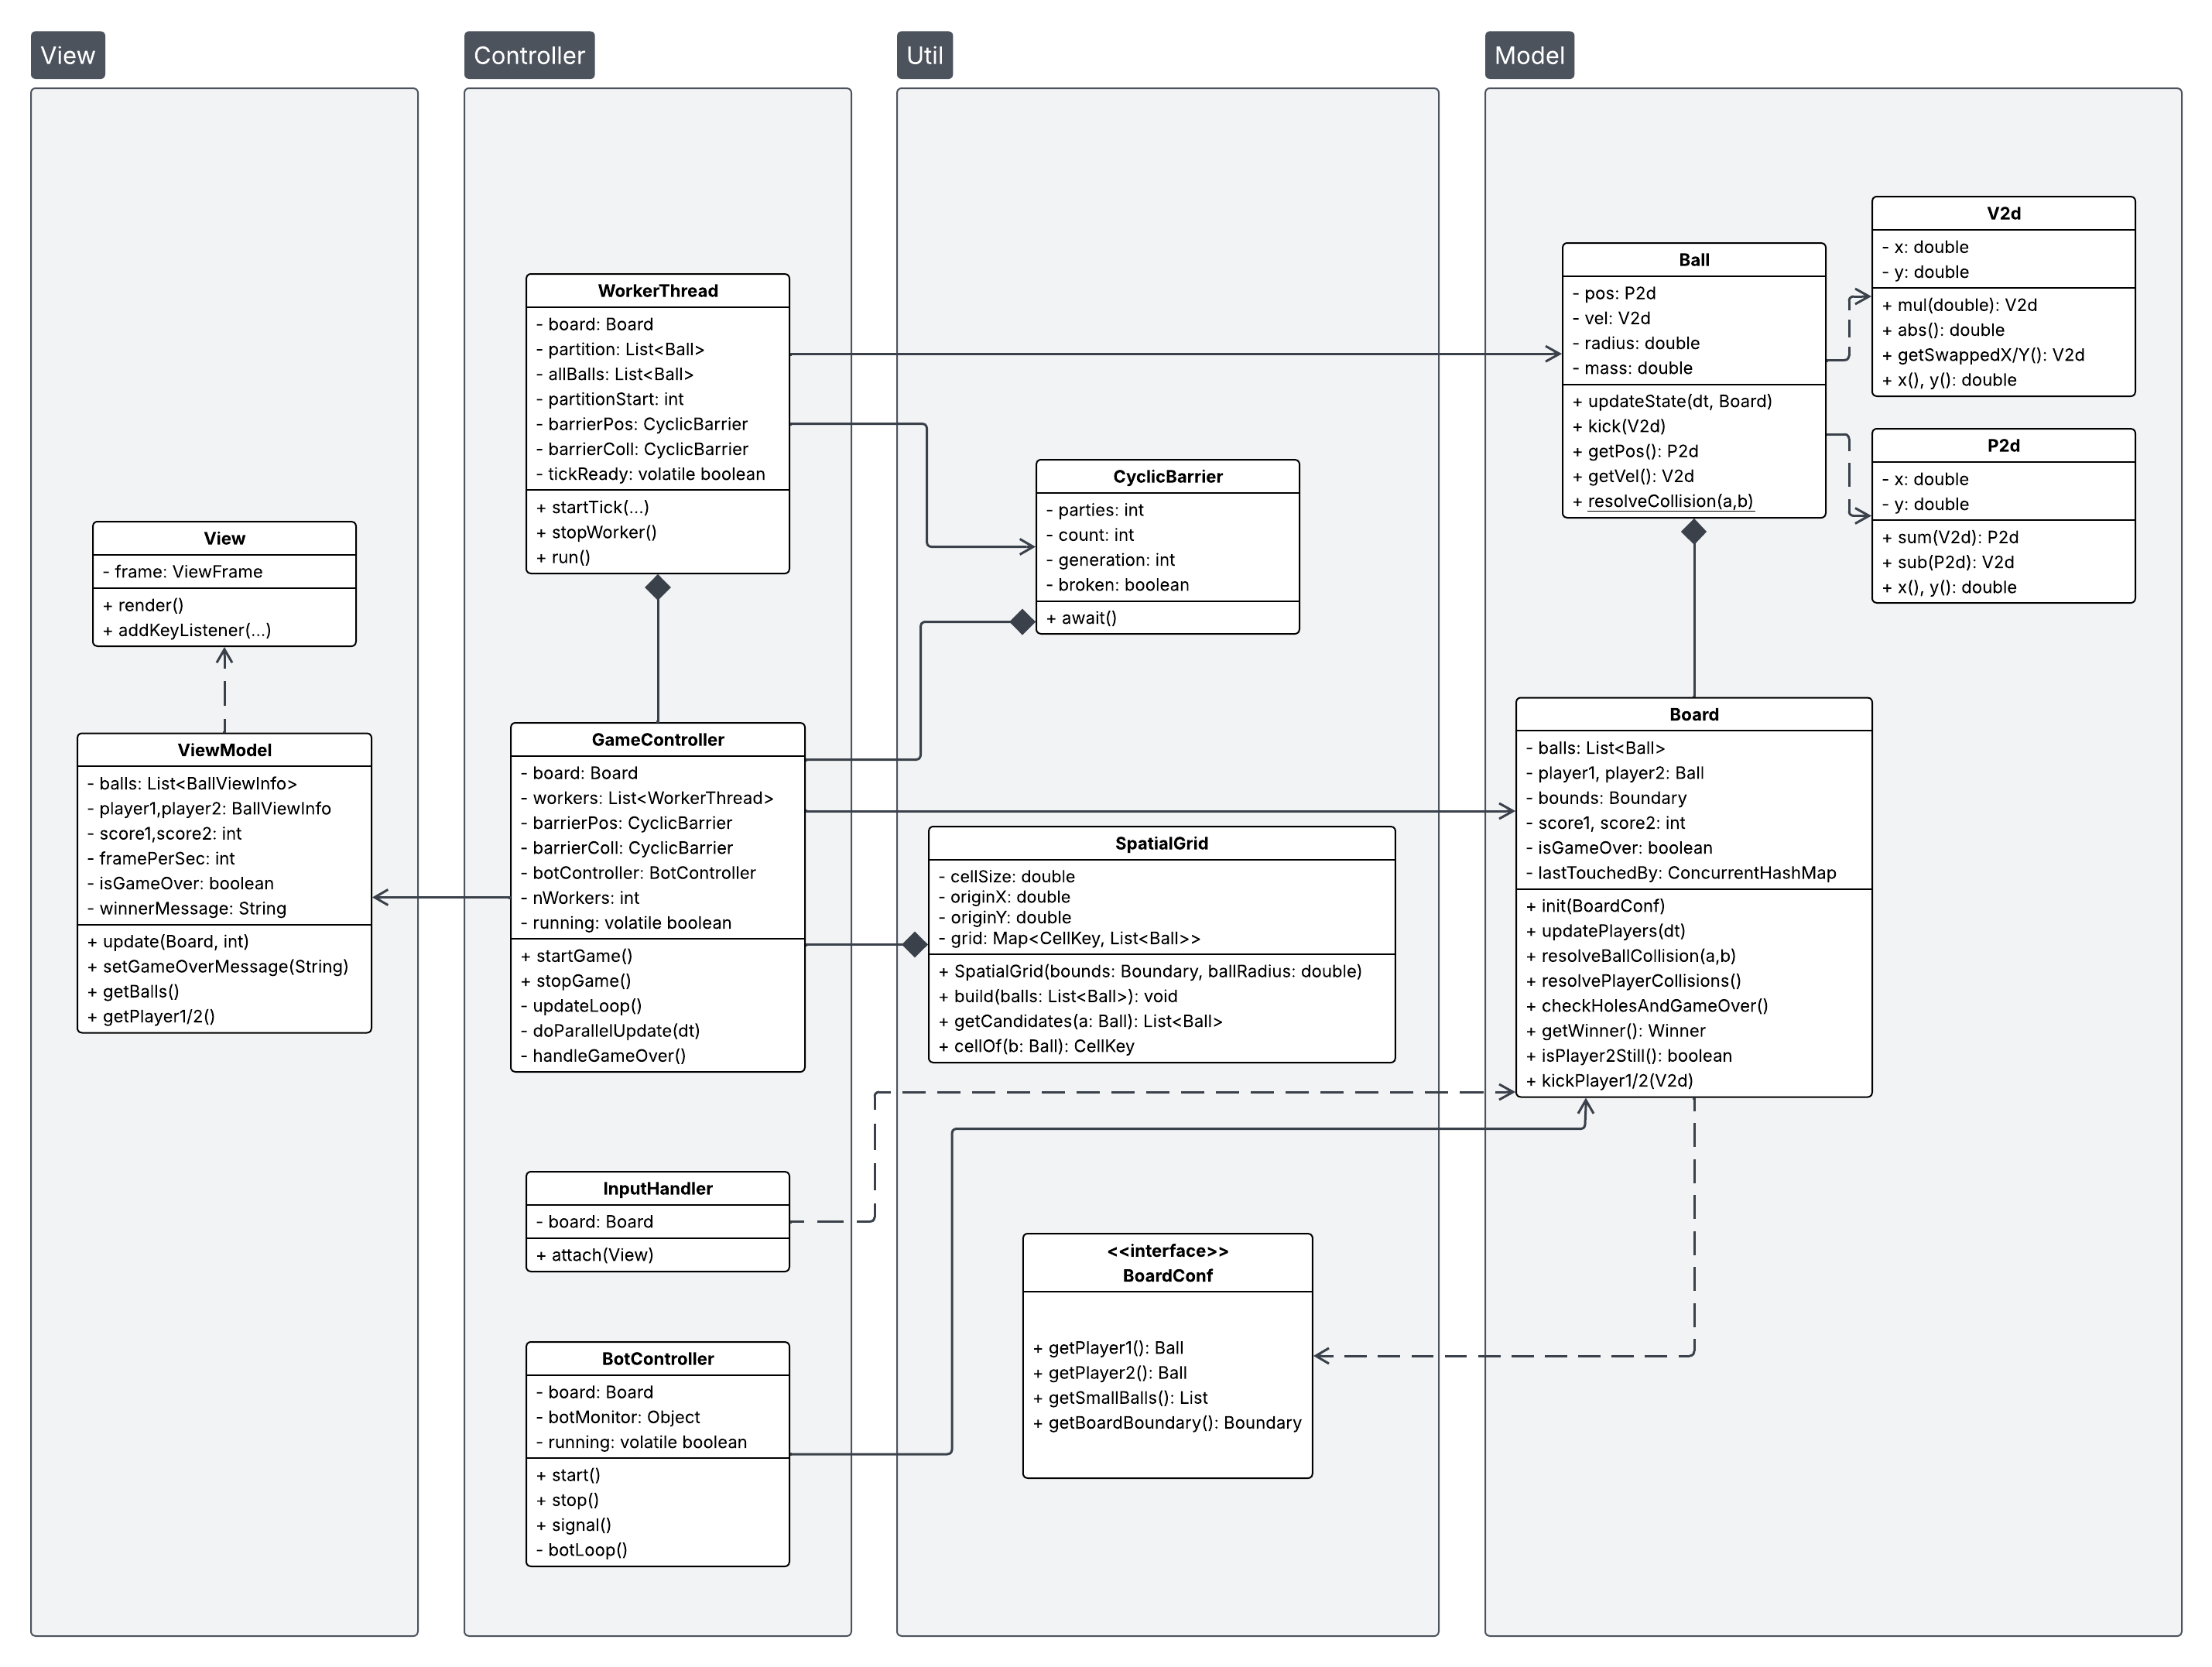
\includegraphics[width=0.8\textwidth]{images/UML_MultiThread.png}
    \caption{UML with MVC graphics subdivision}
    \label{fig:game_flow_petri_net}
\end{figure}
 
% ─────────────────────────────────────────────────────────────────────────────
\subsubsection{Thread Model}
% ─────────────────────────────────────────────────────────────────────────────
 
The application runs five categories of threads simultaneously during a game:
 
\begin{enumerate}
    \item \textbf{Main thread}: bootstraps the model and schedules the Swing
          initialization on the EDT via \texttt{SwingUtilities.invokeLater}.
          It exits immediately after.
 
    \item \textbf{Event Dispatch Thread (EDT)}: It handles key events (forwarded by the Input Handler) and executes
          repaints triggered by \texttt{panel.repaint()}. It never touches
          \texttt{Board} directly: key events call \texttt{board.kickPlayer1()},
          which is \texttt{synchronized}, and repaints read only from
          \texttt{ViewModel}.
 
    \item \textbf{UpdateThread}: a single daemon thread owned by
          \texttt{GameController}. It drives the game loop: it advances the
          physics pipeline each tick, signals \texttt{BotController}, copies
          state into \texttt{ViewModel}, and calls \texttt{view.render()}.
          It also participates in both \texttt{CyclicBarrier}s as the
          $(N+1)$-th party, allowing it to perform the sequential post-barrier
          phases without additional synchronization.
 
    \item \textbf{WorkerThread-0 \ldots WorkerThread-N}: a pool that contains exactly\\ 
          $N = \texttt{availableProcessors()} + 1$ persistent daemon threads,
          created once at startup and never recreated. Each worker waits on its
          private \texttt{tickMonitor} until \texttt{GameController} calls
          \texttt{startTick()}, then executes phase~1 (positions) and phase~2
          (ball-ball collisions) before waiting again for the next tick.
 
    \item \textbf{BotThread}: a single daemon thread owned by
          \texttt{BotController}. It waits on a private \texttt{botMonitor}
          until \texttt{GameController} signals that player~2 is still, then
          applies a random kick impulse subject to a 2-second cooldown.
\end{enumerate}

All threads except the main thread are daemon threads, so the JVM exits cleanly
when the window is closed.
 
% ─────────────────────────────────────────────────────────────────────────────
\subsubsection{Parallel Physics Pipeline}
% ─────────────────────────────────────────────────────────────────────────────
 
The physics update for each game tick is divided into five phases, two of which
execute in parallel across the worker pool.
 
\begin{enumerate}
	\item \textbf{Player update (sequential)}: Before the parallel work begins, \texttt{GameController} calls \texttt{board.updatePlayers(dt)}, which advances the positions of the two heavy player balls. This is sequential because (a) there are only two such balls, and (b) the workers' collision phase reads player state indirectly via \texttt{resolvePlayerCollisions()}, which runs after the barriers. Keeping player updates sequential avoids any contention.
 
	\item \textbf{Position update (parallel)}: The list of small balls is divided into $N$ contiguous, disjoint partitions using a balanced split (each partition differs in size by at most one element). Each \texttt{WorkerThread} receives its partition and calls \texttt{ball.updateState(dt)} on every ball it owns. Because the partitions are disjoint, no two workers write to the same \texttt{Ball} object during this phase, and no locking is required.
 
After finishing, each worker calls \texttt{barrierPositions.await()}. The \texttt{UpdateThread} also calls \texttt{barrierPositions.await()} as the $(N+1)$-th party. The barrier scatters all threads into phase~3 only once every worker (and the controller) has finished phase~2, guaranteeing that all positions are fully updated before any collision is resolved.
 
	\item \textbf{Spatial grid construction (Worker-0 only)}: After all positions have been updated in phase~2, computing ball-ball collisions naively requires checking all $O(n^2)$ pairs. To reduce this to $O(n)$ on average, the application uses a \textbf{spatial hashing grid} implemented in the \texttt{SpatialGrid} class (package \texttt{pcd.assignment01.util}).
 
The field is partitioned into square cells of side $\mathit{cellSize} = 2 \cdot r_{\text{ball}} + \varepsilon$, where $r_{\text{ball}} = 0.01$ is the radius of the small balls. This choice guarantees that two balls whose centres lie in non-adjacent cells have distance $> \mathit{cellSize} > 2 \cdot r_{\text{ball}}$ and therefore cannot overlap: no colliding pair is ever missed by checking only the $3 \times 3$ neighbourhood of cells around each ball.
 
The grid is stored as a \texttt{HashMap<CellKey, List<Ball>>}, where \texttt{CellKey} is a value type wrapping the integer column and row indices of a cell. Using a hash map rather than a dense 2D array avoids allocating memory for the large number of empty cells that arise with sparse ball distributions.
 
The grid must be rebuilt every tick because ball positions change in phase~2. This work is assigned exclusively to \textbf{Worker-0} (\texttt{isGridBuilder == true}), which calls \texttt{grid.build(allBalls)} after \texttt{barrierPositions} has fired.
 
The synchronization for this phase uses a \texttt{ReusableLatch} rather than a \texttt{CyclicBarrier}. The distinction is deliberate: a \texttt{CyclicBarrier} models \emph{symmetric} synchronization — $N$ threads performing parallel work and waiting for each other. Grid construction is instead an \emph{asymmetric} one-to-all dependency: one producer (Worker-0) generates a result that the other workers must wait for before entering phase~4.
 
Worker-0 calls \texttt{gridLatch.open()} after \texttt{grid.build()} completes; all other workers call \texttt{gridLatch.await()} and block until the latch opens. The \texttt{UpdateThread} does not participate in the latch — it proceeds directly from \texttt{barrierPositions} to \texttt{barrierCollisions}. The \texttt{GameController} calls \texttt{gridLatch.reset()} at the start of each tick, before activating any worker, making the latch safely reusable across ticks.
 
The \texttt{open()} call establishes a \emph{happens-before} relationship between Worker-0's writes to the grid and all subsequent reads by the other workers in phase~4, as required by the Java Memory Model.
 
The synchronization points per tick are therefore:
 
\[
\underbrace{\texttt{barrierPositions}}_{\text{symmetric}} \;\to\;
\underbrace{\texttt{gridLatch}}_{\text{asymmetric}} \;\to\;
\underbrace{\texttt{barrierCollisions}}_{\text{symmetric}}
\]
 
The two \texttt{CyclicBarrier} instances are each constructed with $\mathit{parties} = N + 1$ (one per worker plus the \texttt{UpdateThread}). The \texttt{ReusableLatch} has no party count — it is opened by exactly one thread and awaited by all others independently.
 
	\item \textbf{Ball-ball collision resolution with spatial hashing (parallel)}
 
Each worker iterates over its partition and, for each ball~$a$, calls
\texttt{grid.getCandidates(a)} to obtain the balls in the $3 \times 3$ cell
neighbourhood. This returns on average only a small constant number of candidates
(proportional to local ball density) instead of all $n$ balls, reducing the total
work across all workers from $O(n^2)$ to $O(n)$ on average.
 
Each worker also builds a \texttt{Map<Ball, Integer>} index (populated in
\texttt{startTick()}) that maps every ball to its position in the shared
\texttt{allBalls} snapshot. This allows $O(1)$ index lookup during phase~4,
replacing the earlier $O(n)$ \texttt{indexOf()} call that would have negated the
benefit of the spatial grid.
 
The canonical lock-ordering protocol is preserved: a worker processes the pair
$(a, b)$ only if $\mathit{idx}(a) < \mathit{idx}(b)$, ensuring each pair is
handled exactly once across all workers. Locks are acquired in ascending index
order (\texttt{synchronized(a)} then \texttt{synchronized(b)}), which eliminates
the possibility of deadlock by the same argument as before.
 
The performance improvement is significant with dense configurations. With the
\texttt{MassiveBoardConf} (4\,500 balls), the naive $O(n^2)$ approach requires
checking approximately $10^7$ pairs per tick. With the spatial grid, each ball
checks on average fewer than 10 neighbours, reducing the total to roughly
$45\,000$ candidate pairs — a reduction of more than two orders of magnitude.
 
	\item \textbf{Player collision resolution (sequential)}: \texttt{GameController} calls the method
\texttt{board.resolvePlayerCollisions()}, which is \texttt{synchronized} on \texttt{Board}.\\
This method resolves collisions between each player and every small ball, and between the two players themselves. It also updates the \texttt{lastTouchedBy} map, which records the last player to touch each small ball and is used for scoring. This phase is sequential because both player objects are shared across all potential pairs, making fine-grained locking impractical.
 
	\item \textbf{Hole detection and game-over (sequential)}: \texttt{GameController} calls\\
\texttt{board.checkHolesAndGameOver()}, which is also \texttt{synchronized} on \texttt{Board}. It checks whether any ball or player has entered a hole, removes sunk balls from the list, increments scores using \texttt{lastTouchedBy}, and sets \texttt{isGameOver} if appropriate. This phase is sequential because it mutates the shared \texttt{balls} list and the scoring state atomically.
 
\end{enumerate}
 
% ─────────────────────────────────────────────────────────────────────────────
\subsubsection{Synchronization Mechanisms}
% ─────────────────────────────────────────────────────────────────────────────
 
\begin{itemize}
	\item \textbf{CyclicBarrier}
 
The \texttt{CyclicBarrier} (in package \texttt{pcd.assignment01.util}) is
implemented from scratch using Java's built-in monitor protocol
(\texttt{synchronized}, \texttt{wait()}, \texttt{notifyAll()}). It maintains three
fields: \texttt{parties} (the total number of threads that must call \texttt{await()}
before the barrier fires), \texttt{count} (the number of threads still outstanding),
and \texttt{generation} (an integer that increments on each firing and is used as
the condition variable to distinguish the current cycle from the next one, guarding
against spurious wakeups).
 
When the last thread arrives (\texttt{count == 0}), it resets \texttt{count} to
\texttt{parties}, increments \texttt{generation}, and calls \texttt{notifyAll()}.
All waiting threads check \texttt{myGeneration == generation} as their loop
condition: once the generation advances, they know the barrier has fired and they
exit the wait.
 
The barrier also maintains a \texttt{broken} flag. If any waiting thread is
interrupted, it sets \texttt{broken = true} and calls \texttt{notifyAll()}, which
causes every other waiting thread to wake up and throw \texttt{InterruptedException}.
This prevents the pathological scenario where a single interrupted thread leaves
\texttt{count} permanently non-zero, causing all other threads to block forever.
The \texttt{broken} flag is cleared when the last thread successfully fires the
barrier for the next generation.
 
Two instances of \texttt{CyclicBarrier} are created per game, each with
$\mathit{parties} = N + 1$ (one per worker plus the \texttt{UpdateThread}):
\texttt{barrierPositions} separates phase~2 from phase~3, and
\texttt{barrierCollisions} separates phase~4 from the sequential phases~5 and~6.
 
\item \textbf{ReusableLatch}
 
The \texttt{ReusableLatch} (in package \texttt{pcd.assignment01.util}) models
\emph{asymmetric} synchronization: one producer thread calls \texttt{open()} to
signal that a resource is ready, and any number of consumer threads call
\texttt{await()} and block until the latch is open.
 
It is implemented with a single boolean flag \texttt{open} and the standard
monitor protocol. \texttt{await()} loops on \texttt{while (!open) \{ wait(); \}},
and \texttt{open()} sets the flag and calls \texttt{notifyAll()}. The
\texttt{reset()} method closes the latch again for the next cycle; it is called
by the \texttt{GameController} at the start of each tick, before any worker is
activated, so no thread can be in \texttt{await()} at reset time.
 
One instance of \texttt{ReusableLatch} is created per game: \texttt{gridLatch}
gates the transition from phase~3 to phase~4. Worker-0 calls
\texttt{gridLatch.open()} after \texttt{grid.build()} completes; all other workers
call \texttt{gridLatch.await()}. The \texttt{UpdateThread} does not participate in
the latch — it proceeds directly from \texttt{barrierPositions} to
\texttt{barrierCollisions}, since it has no work to do during phase~5.
 
The choice of \texttt{ReusableLatch} over a third \texttt{CyclicBarrier} is
deliberate: a \texttt{CyclicBarrier} implies that all parties perform parallel
work and wait for each other, which would misrepresent the asymmetric nature of
grid construction. Using the semantically correct primitive makes the
synchronization structure of the system explicit and self-documenting.

	\item \textbf{Per-ball locking and deadlock prevention}: During phase~4, each worker acquires \texttt{synchronized} locks on two \texttt{Ball} objects before calling\\
\texttt{Board.resolveBallCollision()}. To prevent deadlock, locks are always acquired in ascending index order (the index of the ball in the shared \texttt{allBalls} snapshot). Because this order is a strict total order and is respected by all workers, no circular wait can occur: a thread holding \texttt{lock(ball[i])} and waiting for \texttt{lock(ball[j])} with $i < j$ will never be blocked by another thread holding \texttt{lock(ball[j])} and waiting for \texttt{lock(ball[i])}.

	\item \textbf{ConcurrentHashMap for \texttt{lastTouchedBy}}: The \texttt{lastTouchedBy} map is accessed from two different contexts: from
\texttt{WorkerThread}s during phase~4 (to remove entries for colliding balls) and
from the \texttt{UpdateThread} during phases~5 and~6 under the \texttt{Board} lock
(to update and query entries). Using a \texttt{ConcurrentHashMap} makes individual
operations on the map thread-safe without requiring a \texttt{synchronized(this)}
block inside \texttt{resolveBallCollision()}. This eliminates a potential deadlock
that would arise from the lock ordering \texttt{synchronized(ball)} $\to$
\texttt{synchronized(board)}, which could interleave incorrectly with
\texttt{synchronized(board)} held by\\
\texttt{resolvePlayerCollisions()}.

	\item \textbf{BotController monitor}: The \texttt{BotController} uses a private \texttt{Object botMonitor} as a condition
variable. The \texttt{BotThread} waits on this monitor inside a guarded loop that
checks both \texttt{running} and \texttt{board.isPlayer2Still()}. The
\texttt{UpdateThread} calls \texttt{botController.signal()} once per tick; if
player~4 is still, \texttt{signal()} calls \texttt{notifyAll()} on the monitor.
The \texttt{stop()} method calls \texttt{notifyAll()} unconditionally, ensuring the
\texttt{BotThread} is always unblocked on shutdown regardless of the ball's current
velocity.

	\item \textbf{ViewModel snapshot and thread safety}: All public methods of \texttt{ViewModel} are \texttt{synchronized} on the
\texttt{ViewModel} instance. The \texttt{UpdateThread} calls \texttt{update()}
once per tick, which replaces the internal collections with fresh copies of the
model state. The EDT calls getters (\texttt{getBalls()}, \texttt{getPlayer1()},
etc.) during repaints. Because \texttt{update()} returns deep copies
(e.g.\ \texttt{new ArrayList<>(balls)}) and all getters return copies as well, the
EDT never holds a reference to an object being mutated by the physics threads.
\end{itemize}
 
% ─────────────────────────────────────────────────────────────────────────────
\subsubsection{MVC and Multithreading Interaction}
% ─────────────────────────────────────────────────────────────────────────────
 
The interaction between the MVC layers in the presence of multiple threads is
governed by three invariants:
 
\begin{enumerate}
    \item \textbf{The Model is only mutated by the controller.}
          The EDT never calls any mutating method on \texttt{Board} except
          \texttt{kickPlayer1()}, which is \texttt{synchronized}. The \texttt{BotThread}
          calls only \texttt{kickPlayer2()}, also \texttt{synchronized}. All physics
          mutations happen exclusively within the sequential and parallel phases
          orchestrated by\\
\texttt{GameController}.
 
    \item \textbf{The View never reads the Model directly.}
          \texttt{ViewFrame} and its inner\\
\texttt{VisualiserPanel} read exclusively
          from \texttt{ViewModel}. The snapshot is written once per tick by the
          \texttt{UpdateThread} after all physics phases are complete, so the view
          always paints a consistent state that reflects a completed tick.
 
    \item \textbf{Game-over handling is atomic with respect to rendering.}
          When\\
\texttt{checkHolesAndGameOver()} sets \texttt{isGameOver = true}, the
          \texttt{UpdateThread} detects this before calling \texttt{viewModel.update()}
          or \texttt{view.render()}.

It calls \texttt{handleGameOver()}, which writes
          the winner message to \texttt{ViewModel} via \texttt{setGameOverMessage()},
          and then renders one final frame. This ensures the game-over overlay is
          shown on a frame that already reflects the final physical state, with no
          intermediate partially-updated frame visible to the player.
\end{enumerate}

\begin{figure}[h]
\centering
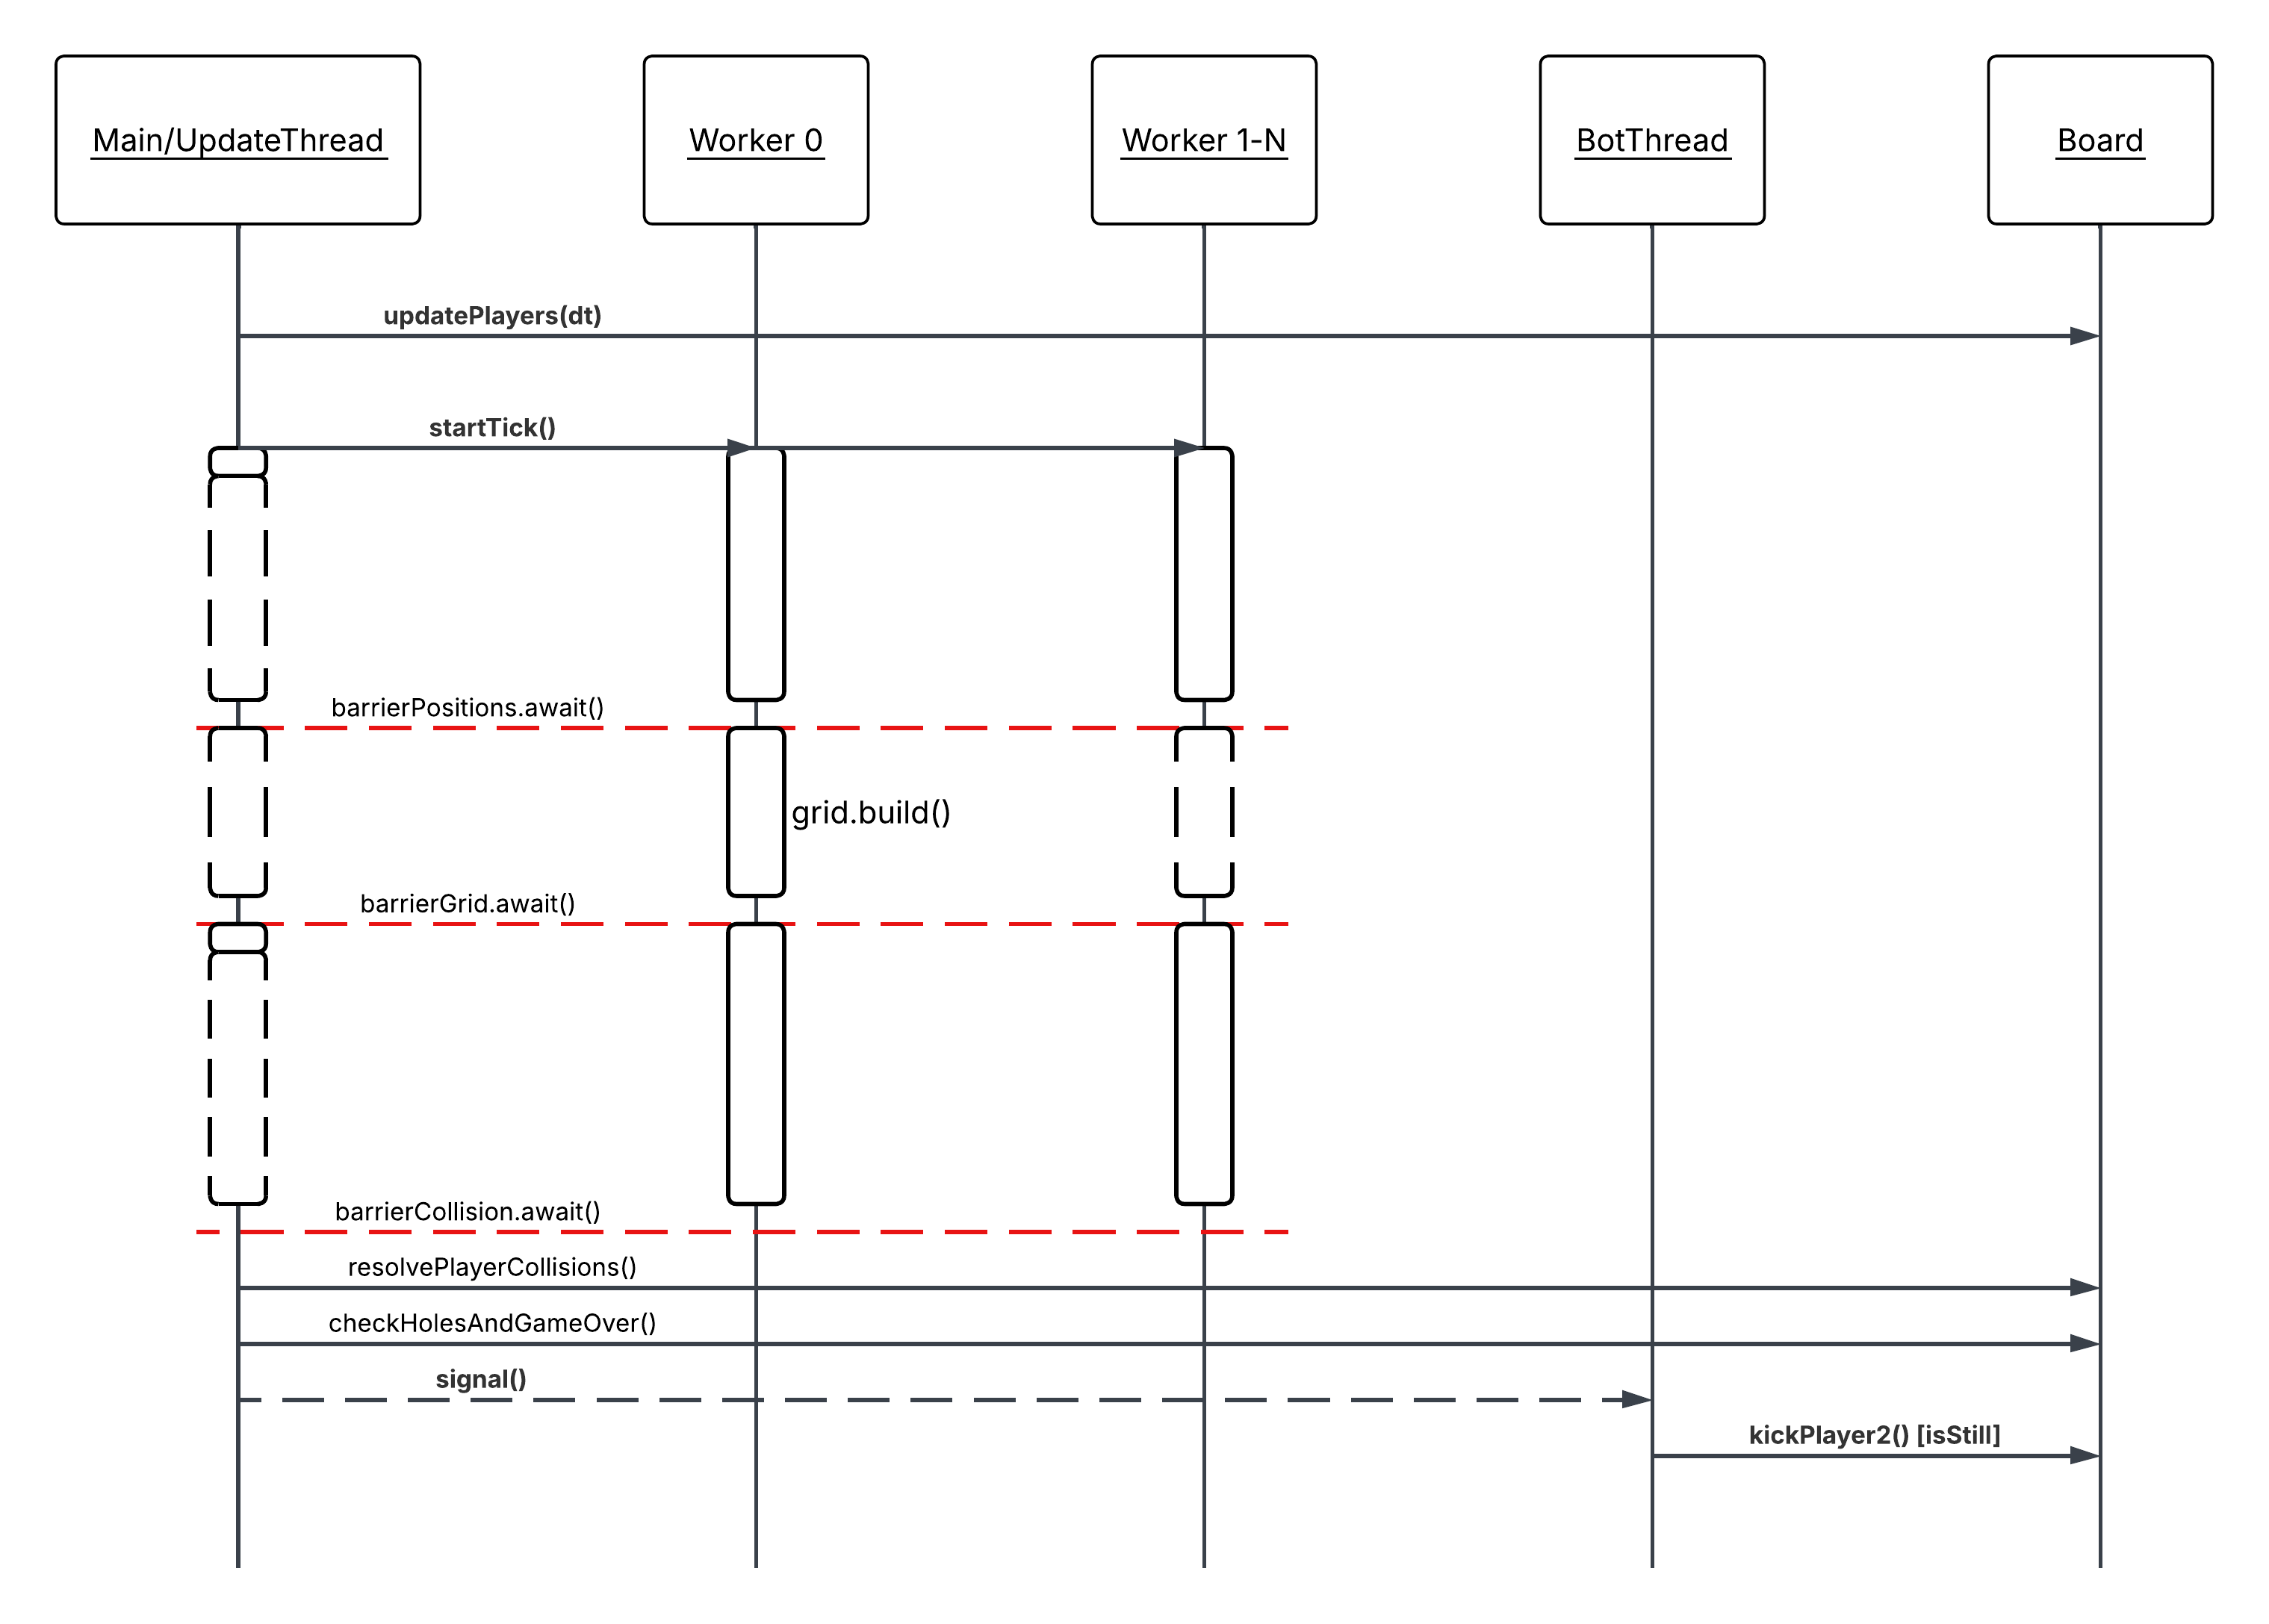
\includegraphics[width=1\textwidth]{images/Sequence Diagram.png}
\caption{Sequence Diagram of thread interactions and synchronization points during a single game tick.}
\label{fig:thread-interaction}
\end{figure}
 
Figure~\ref{fig:thread-interaction} illustrates the interactions between the active threads of the system during a single game tick. Five participants are represented: the \texttt{UpdateThread}, which orchestrates the entire tick; \texttt{WorkerThread-0}, which additionally acts as the spatial grid builder; \texttt{WorkerThread-1..N}, representing all remaining worker threads which behave identically; the \texttt{BotThread}, which operates independently; and \texttt{Board}, included as a passive participant to make explicit which methods are invoked sequentially and by which thread. The Event Dispatch Thread is intentionally omitted, as it interacts with the system exclusively through \texttt{synchronized} methods on \texttt{Board} and \texttt{ViewModel} and does not participate in any of the barrier synchronization points shown.
The diagram covers five phases. In \textbf{Phase 1}, the \texttt{UpdateThread} sequentially calls \texttt{board.updatePlayers(dt)} before any parallel work begins. In \textbf{Phase 2}, the \texttt{UpdateThread} dispatches \texttt{startTick()} to all workers and immediately blocks on \texttt{barrierPositions.await()}, while \texttt{WorkerThread-0} and \texttt{WorkerThread-1..N} update the positions of their respective ball partitions in parallel. The first red dashed line marks the firing of \texttt{barrierPositions}, after which all threads are guaranteed to have completed position updates. In \textbf{Phase 3}, only \texttt{WorkerThread-0} performs work — rebuilding the \texttt{SpatialGrid} from the updated positions — while all other threads block immediately on \texttt{barrierGrid.await()}. The asymmetry in activation box lengths communicates this visually: \texttt{WorkerThread-0} has a tall box while the others have near-zero boxes. The second red dashed line marks the firing of \texttt{barrierGrid}, establishing the happens-before relationship that allows all workers to safely read the grid in the next phase. In \textbf{Phase 4}, all workers resolve ball-ball collisions in parallel using the spatial grid, acquiring per-ball locks in canonical index order to prevent deadlock, while the \texttt{UpdateThread} again blocks immediately. The third red dashed line marks the firing of \texttt{barrierCollisions}. Finally, in \textbf{Phases 5 and 6}, the \texttt{UpdateThread} exclusively calls \texttt{board.resolvePlayerCollisions()} and \texttt{board.checkHolesAndGameOver()} sequentially, then signals the \texttt{BotThread} via \texttt{signal()} before updating the \texttt{ViewModel} and triggering a render.
 


\subsection{Architectural Overview for Task-Based Approach}
The task-based concurrent implementation differs fundamentally 
from the thread-per-entity model. Rather than creating persistent 
threads for each game component, this approach uses the \textbf{Executor Framework}
 with a fixed-size thread pool to parallelize computation-heavy phases of the game loop. 
 We used \textbf{Map-Reduce} algorithms, the architecture implements a Master/Worker 
 pattern where the \texttt{GameLoop} acts as the master coordinator. 
 It delegates tasks to a \texttt{WorkerPool} abstraction which, knowing the data space
  topology in advance, splits the workload into smaller, independent chunks (\textit{map phase}). 
  These chunks are then efficiently computed in parallel by the underlying \texttt{ExecutorService}.
\begin{figure}[h!]
    \centering
    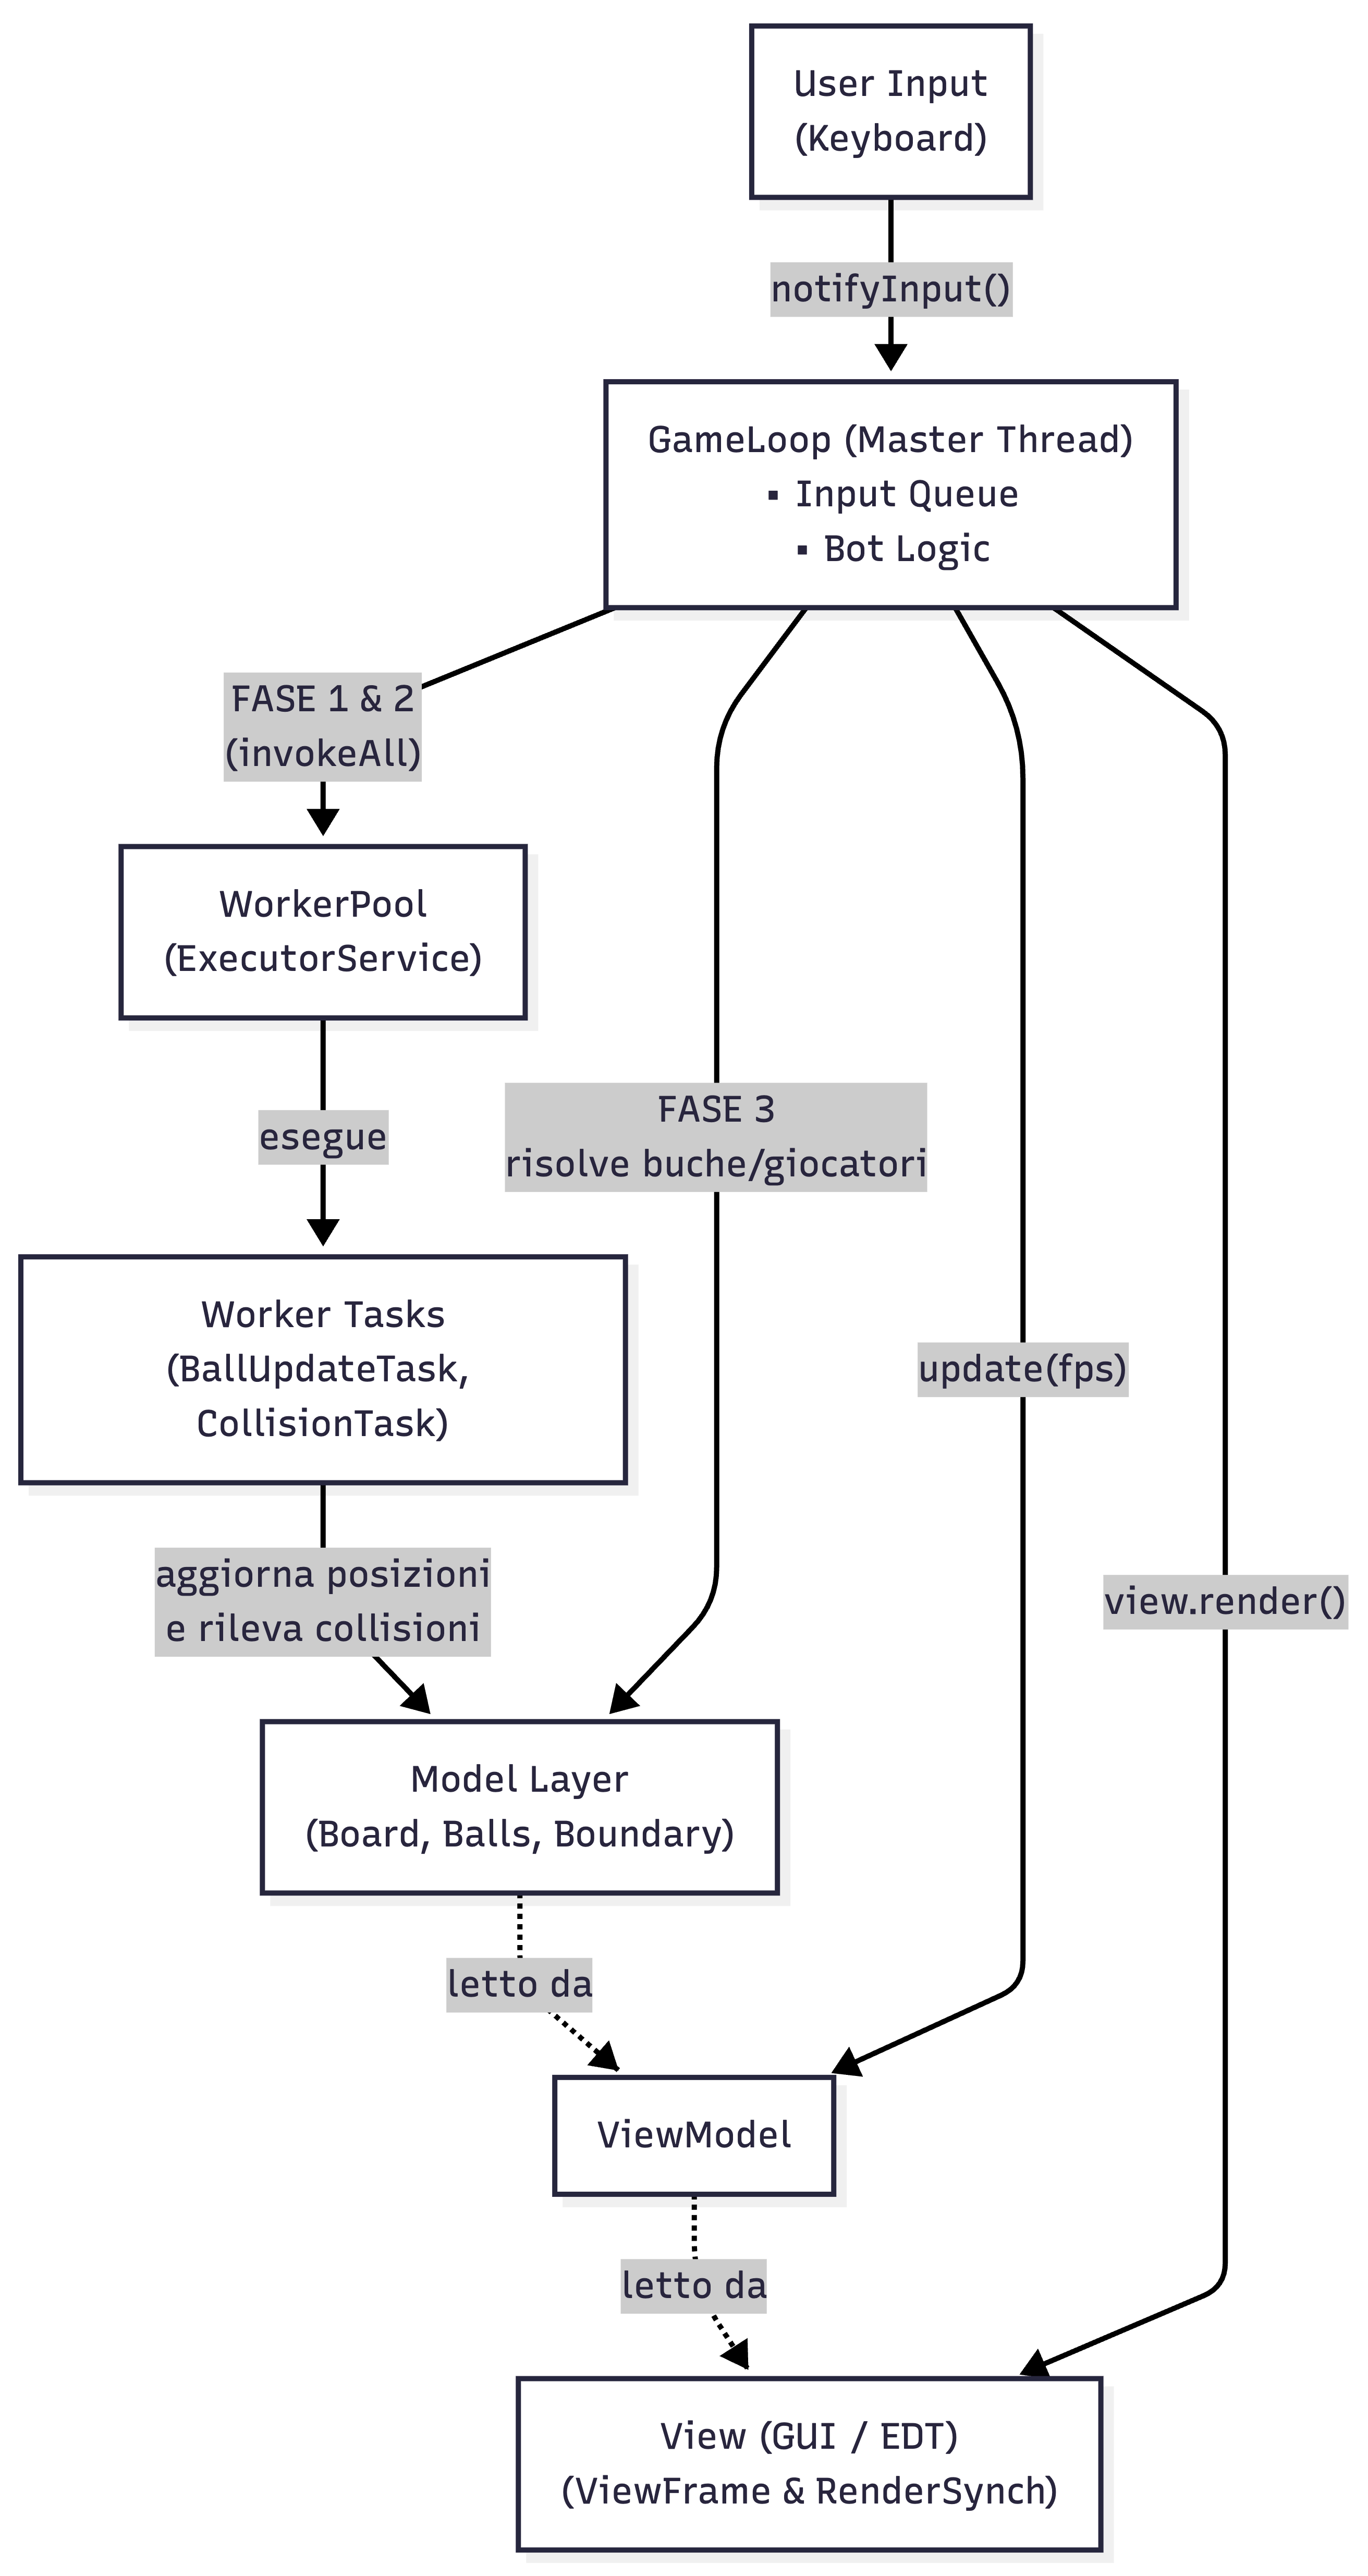
\includegraphics[width=1.1\textwidth]{images/task-based-architecture.png}
    \caption{UML class diagram}
    \label{fig:image_label_1}
\end{figure}

\subsubsection{Component Descriptions}
The task-based architecture consists of the following key components:
 
\subsubsection*{GameLoop (Master/Orchestrator Thread)}
 
The \texttt{GameLoop} extends \texttt{Thread} and serves as the main control flow:
 
\begin{itemize}
    \item \textbf{Role}: Central orchestrator managing game state, input handling, and task delegation
    \item \textbf{Responsibilities}:
    \begin{itemize}
        \item Maintains the main game loop (while !board.isGameOver())
        \item Manages non-blocking input via \texttt{BlockingQueue<V2d> inputQueue}
        \item Delegates parallelizable phases to WorkerPool
        \item Executes sequential phase (player/hole collisions) exclusively
        \item Handles rendering synchronization and frame rate
        \item Catches \texttt{ExecutionException} and \texttt{InterruptedException} from worker tasks
    \end{itemize}
    \item \textbf{Key Code Pattern}:
    \begin{lstlisting}[language=Java, caption=GameLoop Main Loop Structure]
while (!board.isGameOver()) {
    V2d impulse = inputQueue.poll(); // Non-blocking input
    
    // Phase 1: Parallel physics
    workerPool.parallelBallUpdate(board.getBalls(), elapsed, board);
    
    // Sequential player logic
    if (board.getPlayer1() != null) 
        board.getPlayer1().updateState(elapsed, board);
    
    // Phase 2: Parallel collision detection
    workerPool.parallelCollisionDetection(board.getBalls(), 
        board.getLastTouchedBy());
    
    // Phase 3: Parallel player updates 
    workerPool.parallelPlayerCollision();
                
    board.checkHolesAndEndGame();
    
    // Render
    viewModel.update(board, fps);
    view.render();
}
    \end{lstlisting}
\end{itemize}
 
\subsubsection*{WorkerPool (Task Coordinator Abstraction)}
 
The \texttt{WorkerPool} encapsulates all ExecutorService framework details from the GameLoop:
 
\begin{itemize}
    \item \textbf{Role}: Hides complexity of task scheduling, execution, and synchronization
    \item \textbf{Internal Structure}:
    \begin{itemize}
        \item \texttt{ExecutorService executor}: Fixed thread pool with size $k = 2 \times \text{availableProcessors}$
        \item Three public methods: \texttt{parallelBallUpdate()}, \texttt{parallelCollisionDetection()}, and \texttt{parallelPlayerCollision()}
        \item All use \texttt{invokeAll()} for barrier synchronization
    \end{itemize}
    \item \textbf{Key Guarantee}: The GameLoop does not import \texttt{java.util.concurrent.*}, maintaining clean separation of concerns
    \item \textbf{Exception Propagation}: Exceptions in tasks are bundled into \texttt{ExecutionException} and re-thrown at \texttt{f.get()}
\end{itemize}
 
\subsubsection*{BallUpdateTask (Parallel Worker)}
 
Implements \texttt{Callable<Void>} to update a range of balls' physics state:
 
\begin{itemize}
    \item \textbf{Input Parameters}:
    \begin{itemize}
        \item \texttt{List<Ball> balls}: Shared reference to all balls
        \item \texttt{int from, int to}: Range $[from, to)$ of balls this task processes
        \item \texttt{long dt}: Elapsed time since last frame
        \item \texttt{Board board}: Context for boundary constraints
    \end{itemize}
    \item \textbf{Computation}:
    \begin{lstlisting}[language=Java, caption=BallUpdateTask Execution]
public Void call() {
    for (int i = from; i < to; i++) {
        balls.get(i).updateState(dt, board);
    }
    return null;
}
    \end{lstlisting}
    \item \textbf{Synchronization}: No locks required; each task reads from distinct list indices and modifies only the Ball objects at those indices. The Board's boundary data is assumed immutable during execution.
\end{itemize}
 
\subsubsection*{CollisionTask (Parallel Worker)}
 
Implements \texttt{Callable<Void>} to resolve pairwise ball collisions:
 
\begin{itemize}
    \item \textbf{Input Parameters}:
    \begin{itemize}
        \item \texttt{List<Ball> balls}: Shared reference to all balls
        \item \texttt{int from, int to}: Range $[from, to)$ of "first" balls in pairs
        \item \texttt{ConcurrentHashMap<Ball, Integer> lastTouchedBy}: Shared map of ball-to-player touches
    \end{itemize}
    \item \textbf{Pair Enumeration}: For each ball $i \in [from, to)$, checks pairs $(i, j)$ where $j \in [i+1, n)$
    \item \textbf{Synchronization Protocol}:
    \begin{lstlisting}[language=Java, caption=Ordered Lock Acquisition in CollisionTask]
for (int i = from; i < to; i++) {
    for (int j = i + 1; j < n; j++) {
        Ball a = balls.get(i);
        Ball b = balls.get(j);
        
        // Ordered lock acquisition (deadlock prevention)
        Ball first = System.identityHashCode(a) <= System.identityHashCode(b) ? a : b;
        Ball second = (first == a) ? b : a;
        
        synchronized (first) {
            synchronized (second) {
                Ball.resolveCollision(a, b);
                // Update lastTouchedBy if collision occurred
                if (velocities changed) {
                    lastTouchedBy.put(a, 0);
                    lastTouchedBy.put(b, 0);
                }
            }
        }
    }
}
    \end{lstlisting}
    \item \textbf{Fine-Grained Locking}: Each pair's collision resolution is protected by locks on both Ball objects, but independent pairs may execute concurrently.
\end{itemize}

\subsubsection*{PlayerCollisionTask (Parallel Worker)}
Implements \texttt{Callable<Void>} to resolve player-ball collisions in parallel:
\begin{itemize}
    \item \textbf{Input Parameters}:
    \begin{itemize}
        \item \texttt{List<Ball> balls}: Shared reference to all balls
        \item \texttt{int from, int to}: Range $[from, to)$ of "first" balls in pairs
        \item \texttt{ConcurrentHashMap<Ball, Integer> lastTouchedBy}: Shared map of ball-to-player touches
    \end{itemize}
    \item \textbf{Pair Enumeration}: For each ball $i \in [from, to)$, checks pairs $(i, j)$ where $j \in [i+1, n)$
    \item \textbf{Synchronization Protocol}:
    \begin{lstlisting}[language=Java, caption=Ordered Lock Acquisition in PlayerCollisionTask]
for (int i = from; i < to; i++) {
            Ball b = balls.get(i);

            // Collisione con player1
            if (player1 != null) {
                V2d vPrima = b.getVel();
                Ball.resolveCollision(player1, b);
                if (!b.getVel().equals(vPrima)) {
                    lastTouchedBy.put(b, 1);
                }
            }

            // Collisione con player2
            if (player2 != null) {
                V2d vPrima = b.getVel();
                Ball.resolveCollision(player2, b);
                if (!b.getVel().equals(vPrima)) {
                    lastTouchedBy.put(b, 2);
                }
            }
        }
        return null;
    \end{lstlisting}

\end{itemize}
 
\subsubsection*{Task Decomposition}
Task decomposition in the Poool implementation follows a \textbf{range-partitioning} strategy:
 
\begin{itemize}
    \item \textbf{Chunk Size Calculation}:
    \begin{lstlisting}[language=Java, caption=Chunk Size Computation in WorkerPool]
int nWorkers = Runtime.getRuntime().availableProcessors() * 2;
int chunkSize = Math.max(1, n / nWorkers);
    \end{lstlisting}
    where $n$ is the number of balls. This ensures:
    \begin{itemize}
        \item If $n = 4500$ balls and $k = 8$ cores (16 workers), chunk size $\approx 281$ balls per task
        \item Minimum chunk size of 1 prevents empty tasks
        \item Factor of 2 overprovisioning creates more granularity for load balancing
    \end{itemize}
\end{itemize}

\subsection{Synchronization Strategy}
Task-based synchronization employs a layered strategy combining barrier synchronization with fine-grained locking:
 
\subsubsection{Barrier Synchronization via invokeAll()}
 
Parallel phases use \texttt{ExecutorService.invokeAll()}, which provides implicit barrier semantics:
 
\begin{itemize}
    \item \textbf{Behavior}: Blocks until \textit{all} submitted tasks complete
    \item \textbf{Java Memory Model Guarantee}: All field writes in tasks are visible after invokeAll() returns (happens-before relationship)
    \item \textbf{Game Loop Implications}:
    \begin{itemize}
        \item Phase 1 completes $\implies$ all ball positions/velocities updated and visible
        \item Phase 2 completes $\implies$ all collision resolutions applied and visible
        \item Phase 3 completes $\implies$ all player updates applied and visible
        \item Sequential Phase 4 executes with consistent global state
    \end{itemize}
    \item \textbf{Performance Cost}: Tail latency --- the slowest task determines phase duration
\end{itemize}
 
\subsubsection{Fine-Grained Ball Locking in Collision Detection}
 
CollisionTask uses nested synchronized blocks to prevent data races during collision resolution:
 
\begin{itemize}
    \item \textbf{Two Locks}: Each \texttt{Ball.resolveCollision(a, b)} modifies both Ball objects' velocity and position. Without synchronization, a concurrent update might corrupt the ball state.
    \item \textbf{Deadlock Prevention via Ordering}:
    \begin{itemize}
        \item All code acquires locks in a consistent order: always lock Ball A before Ball B if identityHashCode(A) $\leq$ identityHashCode(B)
        \item Since identity hash codes are fixed per object, this prevents circular wait (requirement for deadlock)
    \end{itemize}
    \item \textbf{Lock Contention}: Multiple tasks may compete for the same Ball locks
    \begin{itemize}
        \item If two tasks both need to resolve collisions involving the same Ball, one task waits
        \item This serializes independent collisions unnecessarily, but ensures safety
        \item In practice, contention is moderate since each task processes a different range of "first" balls
    \end{itemize}
\end{itemize}
 
\subsubsection{ConcurrentHashMap for Shared State}
 
The \texttt{lastTouchedBy} map is a \texttt{ConcurrentHashMap<Ball, Integer>} to allow concurrent updates from multiple CollisionTask instances:
 
\begin{itemize}
    \item \textbf{Concurrent Put Operations}: Multiple tasks call \texttt{lastTouchedBy.put(ball, 0)} simultaneously
    \item \textbf{Bucket-Level Locking}: ConcurrentHashMap uses segment-based locking (in modern Java, striped locking)
    \begin{itemize}
        \item Reduces contention compared to a single global synchronized lock
        \item Different Ball keys typically hash to different buckets, allowing concurrent puts
        \item Same-bucket updates still serialize
    \end{itemize}
    \item \textbf{Visibility Guarantee}: All puts are visible globally via ConcurrentHashMap's internal synchronization
\end{itemize}
 
\subsubsection{Exception Handling and Reliability}
 
Task-based execution requires careful exception handling to prevent loop crashes:
 
\begin{itemize}
    \item \textbf{ExecutionException}: If a task throws an unchecked exception, \texttt{f.get()} re-throws it wrapped in ExecutionException
    \item \textbf{InterruptedException}: If the GameLoop thread is interrupted (e.g., window closed), waiting on futures throws InterruptedException
    \item \textbf{GameLoop Protection}:
    \begin{lstlisting}[language=Java, caption=Exception Handling in GameLoop]
try {
    workerPool.parallelBallUpdate(board.getBalls(), elapsed, board);
    workerPool.parallelCollisionDetection(board.getBalls(), 
        board.getLastTouchedBy());
    workerPool.parallelPlayerCollision();
} catch (InterruptedException | ExecutionException e) {
    Thread.currentThread().interrupt();
    break; // Exit game loop gracefully
}
    \end{lstlisting}
    \item \textbf{Graceful Degradation}: Catching exceptions allows the game loop to terminate cleanly rather than crashing the entire JVM
\end{itemize}
 
\subsubsection{Memory Visibility and Happens-Before Guarantees}
 
The Java Memory Model ensures correctness through explicit synchronization points:
 
\begin{enumerate}
    \item \textbf{Task Submission}: When a task is submitted to the executor, all field writes in the GameLoop thread are visible to the task
    \item \textbf{Task Execution}: Workers read shared Ball objects and Board state; without locks, visibility is not guaranteed
    \item \textbf{invokeAll() Barrier}: When invokeAll() returns, all task writes are visible to the GameLoop thread
    \item \textbf{Nested Locks in Collisions}: Each \texttt{synchronized} block creates a memory barrier, ensuring Ball field updates are visible across tasks
\end{enumerate}
 
This ensures that despite the distributed nature of tasks, the game state remains consistent across phase boundaries.
 

\section{Behavior Specification: Petri Nets}

% ─────────────────────────────────────────────────────────────────────────────
\subsection{Multi-Threaded CyclicBarrier Net}
% ─────────────────────────────────────────────────────────────────────────────

The \texttt{CyclicBarrier} is a custom synchronization primitive implemented
from scratch. Modelling it as a Petri Net allows its correctness properties —
absence of deadlock, liveness, and automatic reset — to be verified
independently of the application logic that uses it.
 
The net represents a generic barrier with $N+1$ parties, where $N$ is the
number of worker threads. Two representative rows are shown explicitly (Thread~0
and Thread~$N{+}1$), with the intermediate threads indicated by the vertical
ellipsis ($\vdots$). Each thread is modelled by three places: \textit{free}
(initial state, carries the initial token), \textit{wait} (the thread has
called \texttt{await()} and is blocked), and \textit{done} (the thread has
been released by the barrier and is proceeding). The arc from \textit{done}
back to \textit{free} models the cyclic reset: after each tick the thread
returns to its initial state, ready for the next barrier cycle.
 
The single vertical transition \textit{barrier fires} is the core of the net.
It has $N+1$ incoming arcs — one from each \textit{wait} place — and $N+1$
outgoing arcs — one to each \textit{done} place. It is enabled if and only if
all $N+1$ \textit{wait} places simultaneously hold a token, which corresponds
exactly to the condition \texttt{count == 0} in the Java implementation.
 
\begin{figure}[h]
\centering
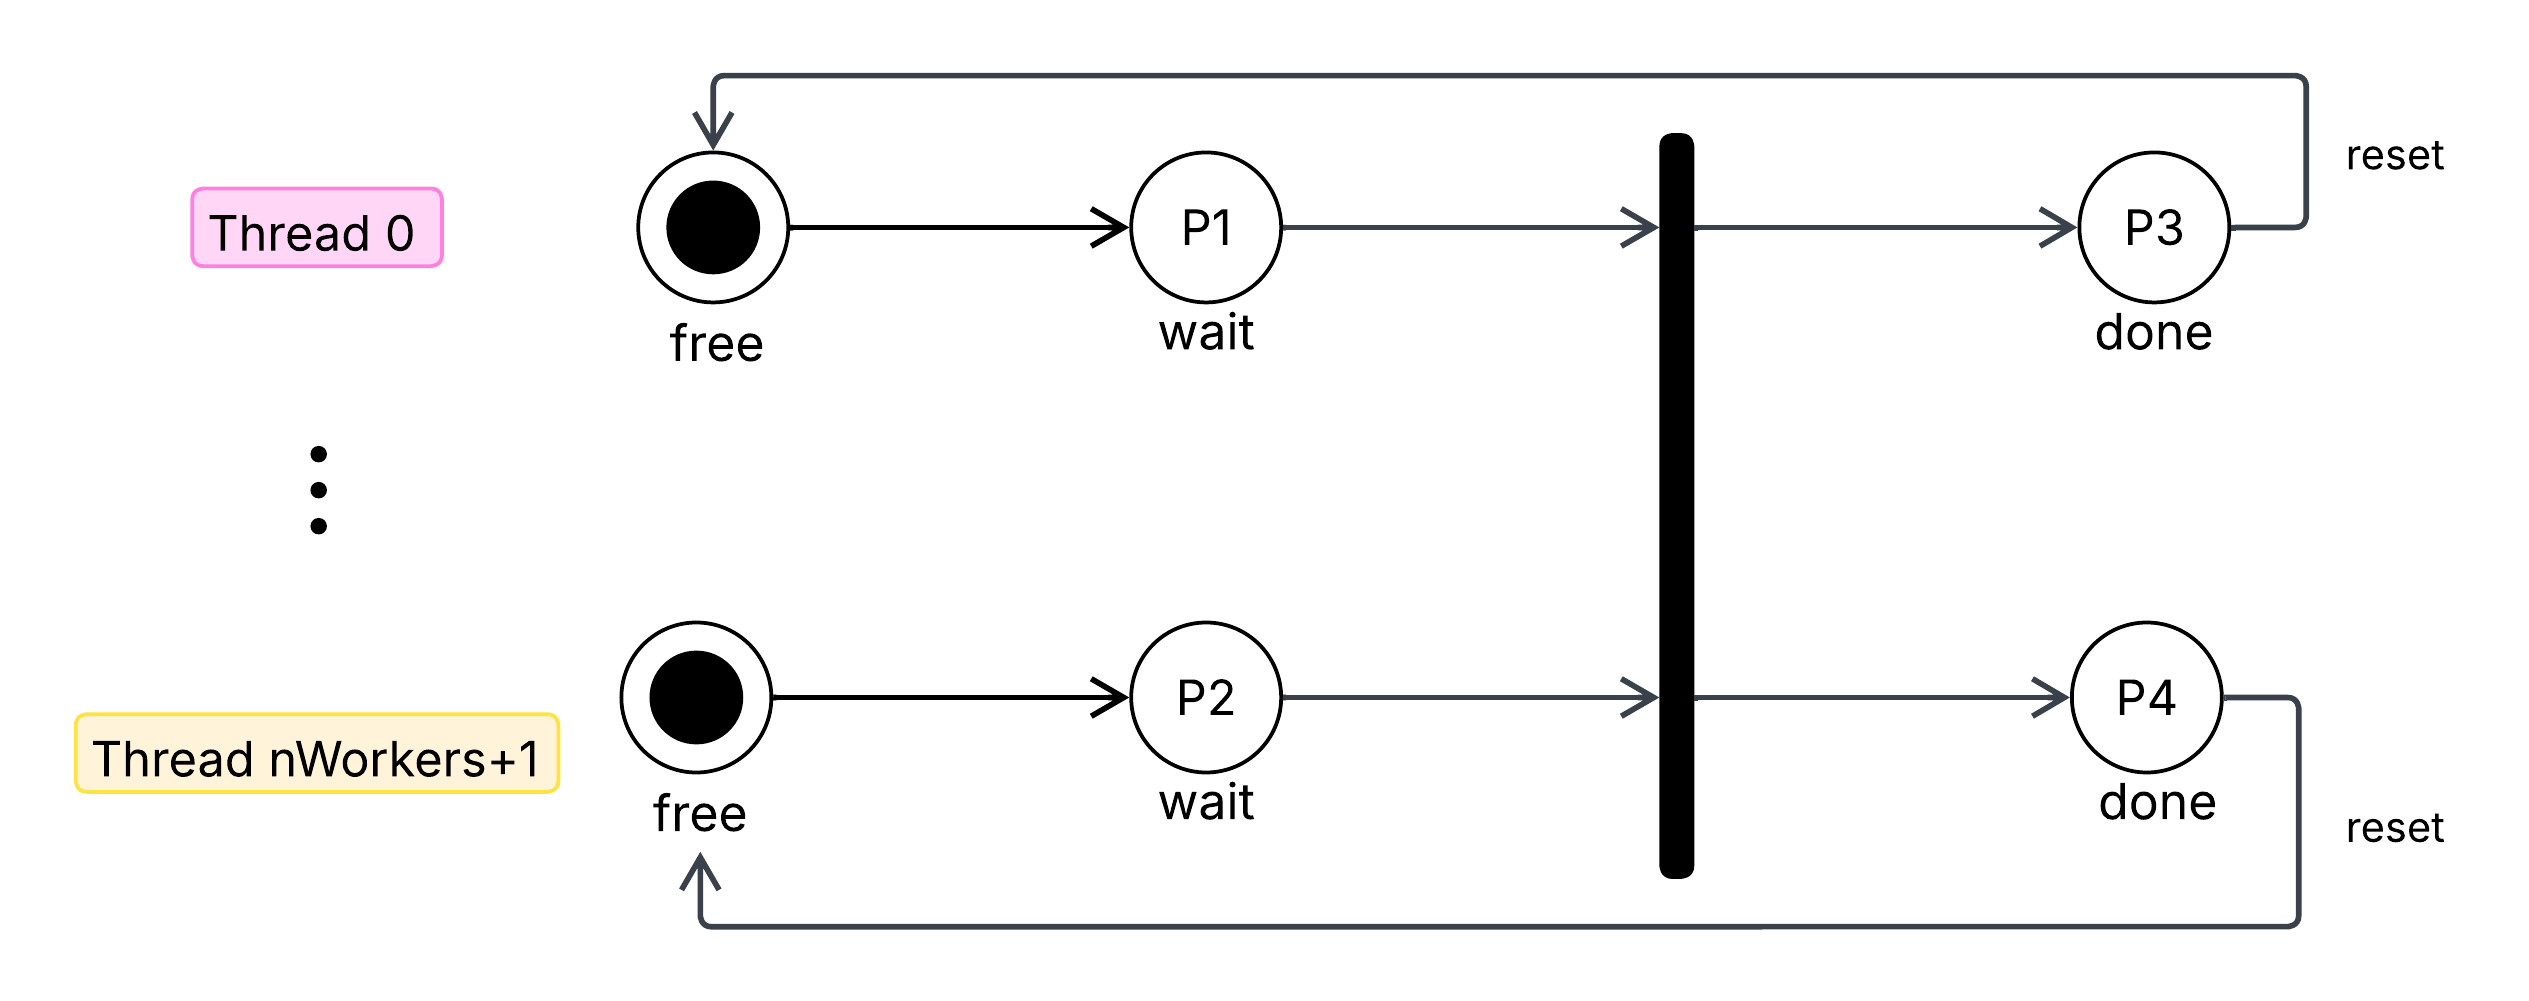
\includegraphics[width=0.75\textwidth]{images/petri_cyclic_barrier.png}
\caption{Petri Net modelling the \texttt{CyclicBarrier} with $N+1$ parties.
         Thread~0 and Thread~$N{+}1$ are shown explicitly; intermediate threads
         follow the same structure. The transition \textit{barrier fires} is
         enabled only when all \textit{wait} places hold a token simultaneously.}
\label{fig:petri-barrier}
\end{figure}
 
The key properties visible from the net structure are the following.
 
\textbf{Absence of deadlock.} The transition \textit{barrier fires} is enabled
if and only if every thread has deposited its token in its \textit{wait} place.
Since each thread has no alternative path that bypasses \textit{wait}, every
token will eventually arrive there, guaranteeing that the transition fires. No
subset of threads can block the others indefinitely.
 
\textbf{Liveness.} After \textit{barrier fires}, every \textit{done} place
receives a token, releasing all threads simultaneously. The net is live: in
any fair execution, every reachable marking eventually leads to the barrier
firing and all threads proceeding.
 
\textbf{Cyclic reset.} The arc from \textit{done} back to \textit{free}
restores the initial marking after each cycle, making the barrier reusable
across ticks without reallocation. This corresponds to the \texttt{generation}
counter and the \texttt{count} reset in the Java implementation.
 
\textbf{Boundedness.} The net is 1-safe: at most one token resides in any
place at any time. Each thread produces exactly one token per cycle, the
transition consumes all tokens atomically, and the loop arc returns exactly
one token to \textit{free}. No accumulation is possible.

% ─────────────────────────────────────────────────────────────────────────────
\subsection{Multi-Threaded Tick Flow}
% ─────────────────────────────────────────────────────────────────────────────

The second net models the complete flow of a single game tick across all active
threads: the \texttt{UpdateThread}, \texttt{WorkerThread-0},
\texttt{WorkerThread-1..N}, and the \texttt{BotThread}. Each thread is
represented as a horizontal row of places connected by transitions; vertical
transitions that span multiple rows model synchronization points between threads.

\begin{figure}[h]
\centering
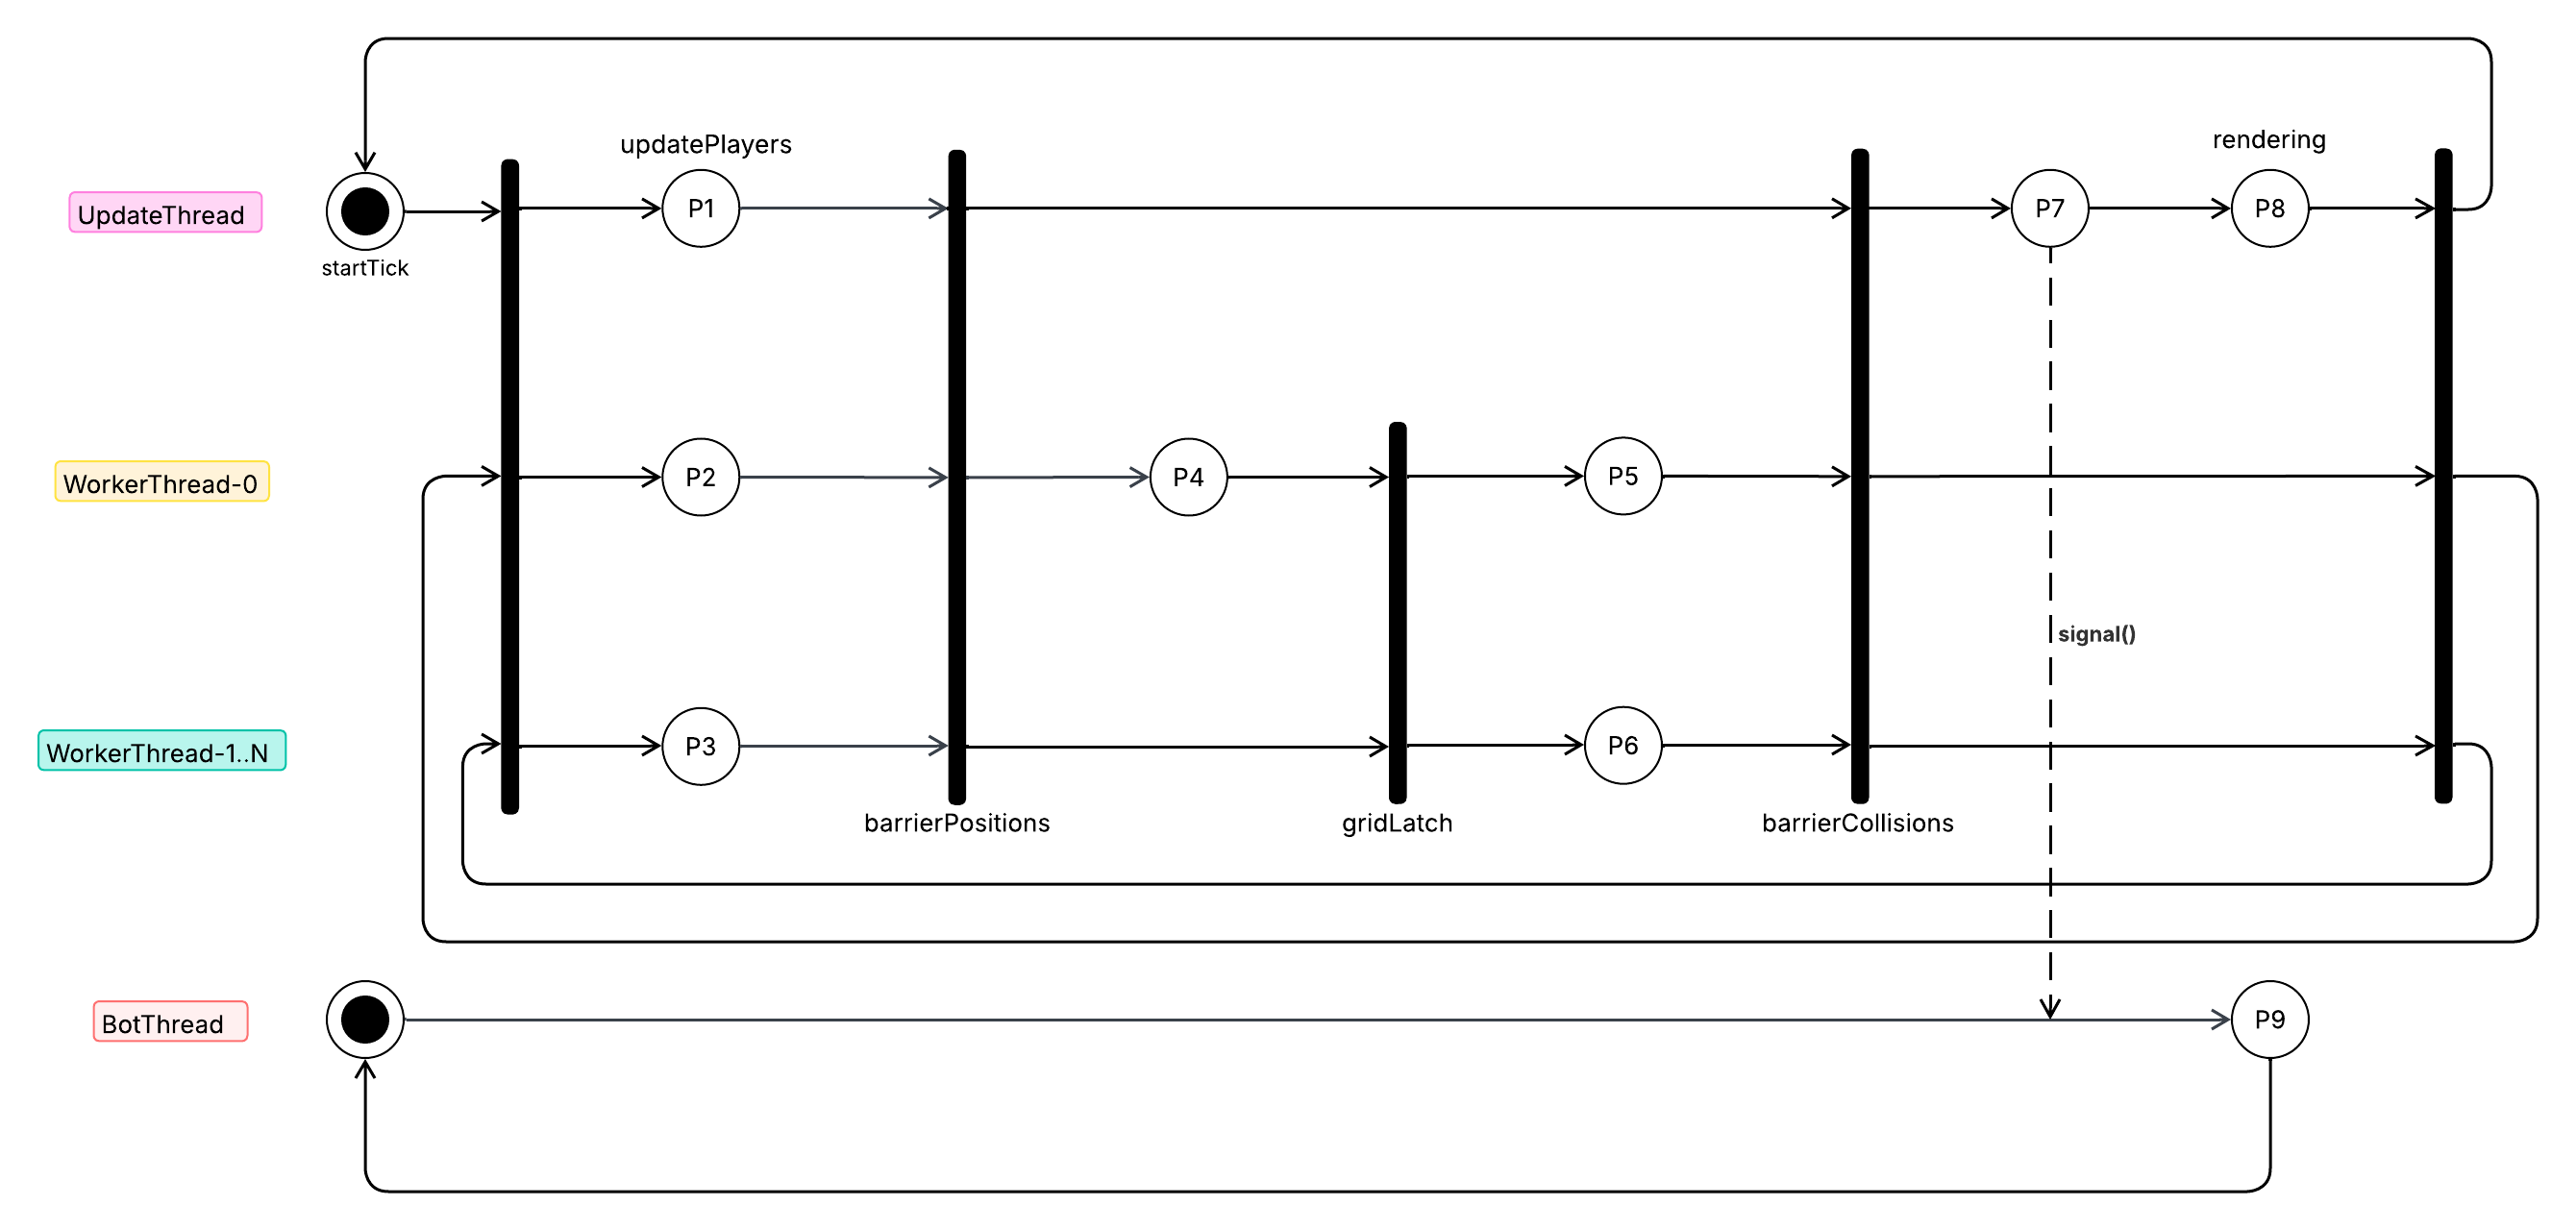
\includegraphics[width=\textwidth]{images/Petri_net_tick_flow.png}
\caption{Petri Net modelling the per-thread state flow during a single game tick.
         Vertical transitions crossing multiple rows represent synchronization
         points. The \texttt{gridLatch} transition spans only the worker rows,
         reflecting its asymmetric producer-consumer semantics.}
\label{fig:petri-tick}
\end{figure}

\textbf{Thread states.} Each place in the net represents a meaningful state
of the corresponding thread. For the \texttt{UpdateThread}: \textit{tick start},
\textit{update players}, \textit{await barrierGrid}, \textit{sequential phases},
\textit{rendering}, and \textit{tick done}. For \texttt{WorkerThread-0}:
\textit{await startTick}, \textit{phase~1}, \textit{grid build}, \textit{phase~2},
and \textit{await next tick}. For \texttt{WorkerThread-1..N}: the same sequence
except that \textit{grid build} is replaced by a direct arc from
\texttt{barrierPositions} to \texttt{gridLatch}, reflecting the absence of any
work during phase~G. For the \texttt{BotThread}: \textit{await signal} and
\textit{kick (if still)}.

\textbf{Symmetric synchronization — \texttt{barrierPositions} and
\texttt{barrierCollisions}.} These two transitions span the rows of all three
physics threads (\texttt{UpdateThread},\\
\texttt{WorkerThread-0}, and
\texttt{WorkerThread-1..N}). Each is enabled only when all three rows
simultaneously hold a token in the corresponding input place, modelling the
all-to-all semantics of the \texttt{CyclicBarrier}: every thread must complete
its current phase before any thread may advance to the next.

\textbf{Asymmetric synchronization — \texttt{gridLatch}.} This transition spans
only the two worker rows, not the \texttt{UpdateThread} row. Its semantics differ
fundamentally from those of the two barriers: it models a one-to-all dependency
where \texttt{WorkerThread-0} (the producer) opens the latch after
\texttt{grid.build()} completes, and \texttt{WorkerThread-1..N} (the consumers)
are unblocked. The \texttt{UpdateThread} bypasses the latch entirely, proceeding
directly from \texttt{barrierPositions} to \texttt{barrierCollisions} via its own
arc. The asymmetry is visible in the net structure: \texttt{WorkerThread-0} has an
intermediate place \textit{grid build} before the \texttt{gridLatch} transition,
while \texttt{WorkerThread-1..N} has no such place, reflecting that only Worker-0
performs work during phase~G.

\textbf{BotThread independence.} The \texttt{BotThread} row is decoupled from
the physics rows: it has no shared transitions with the barrier or latch
synchronization points. It is connected to the rest of the net only by the
dashed \texttt{signal()} arc from the \texttt{UpdateThread}, which fires after
\texttt{barrierCollisions} and triggers the bot's kick transition if\\
\texttt{isPlayer2Still()} holds. This independence is a deliberate design choice:
the bot must not interfere with the physics pipeline timing.

\textbf{Behavioral properties.} The net is 1-safe and live by the same argument
as the \texttt{CyclicBarrier} net: every thread row has exactly one token in
circulation at any time, and every synchronization transition is eventually
enabled because no thread has an alternative path that bypasses a barrier or the
latch. The loop arcs returning each thread to its initial place after a completed
tick confirm that the system can execute indefinitely without reaching a dead
marking, consistent with the \texttt{no errors detected} result from JPF
verification.

\subsection{High-Level Game Flow Net Task-based}
The system can be broken down into actions called “tasks”; agents are responsible 
for carrying them out. The computations required to complete each 
individual task can occur in parallel; however, there are temporal
 dependencies within the system. The sequential nature of the problem is 
 fundamentally due to the data dependencies between tasks: if a variable 
 must be read in order to complete a task, then it must be ensured that this 
 variable does not change during the read operation, so as not to lose information.

\vspace{1.5em}

\begin{tabular}{ |p{5cm}|p{5cm}|p{5cm}|  }
\hline
Tasks & Temporal Dependencies & Data Dependencies \\
\hline
Ball Update & Must complete BEFORE Collision Detection & Reads: position, velocity, bounds, elapsed time. Writes: updated position, velocity \\
\hline
Collision Update & Starts AFTER Ball Update barrier; Completes BEFORE Player Collision barrier   & Reads: position, velocity, radius, mass (all balls), lastTouchedBy. Writes: velocity, position, lastTouchedBy \\
\hline
Player Collision & Starts AFTER Collision Detection barrier; Completes BEFORE Rendering & Reads: position, velocity, player positions, bounds, lastTouchedBy, scores. Writes: velocity, position, lastTouchedBy, scores, balls list, isGameOver, winnerMessage \\
\hline
Simulation Rendering    & Starts AFTER Player Collision; Completes BEFORE next frame input poll & Reads: balls list, player positions, scores, isGameOver, winnerMessage, framePerSec. Writes: ViewModel state, GUI rendering \\
\hline
\end{tabular}

\vspace{1.5em}

By following the table, it is possible to represent the basic behavior of the system using
a generic Petri net, which is ideally suited for representing the temporal dependencies
of individual tasks.

\begin{figure}[h!]
    \centering
    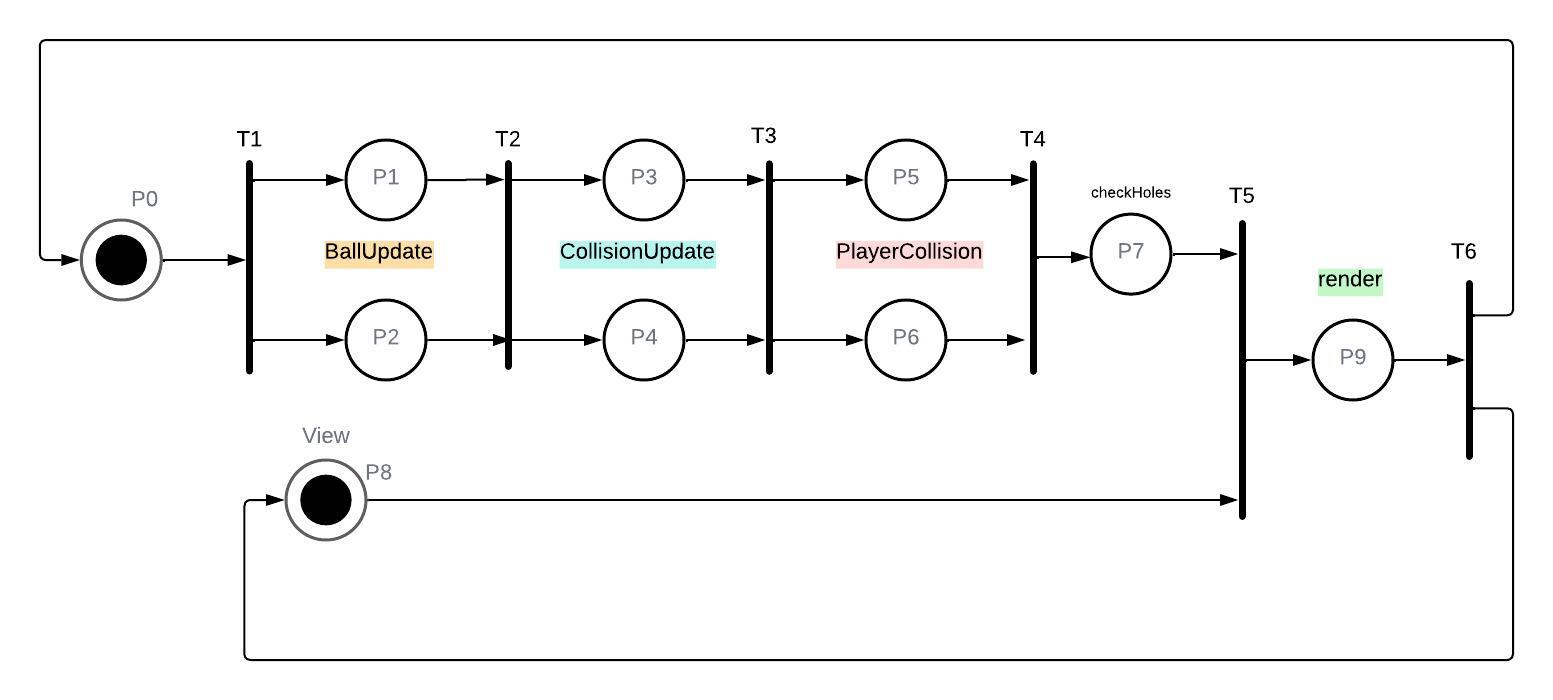
\includegraphics[width=0.8\textwidth]{images/Petri_net_ass_1.jpeg}
    \caption{High-Level Game Flow Petri Net}
    \label{fig:game_flow_petri_net}
\end{figure}





% ─────────────────────────────────────────────────────────────────────────────
\section{Performance Evaluation}
% ─────────────────────────────────────────────────────────────────────────────

This chapter evaluates the runtime performance of the two concurrent
implementations of the Poool simulation. Both versions are designed to
exploit hardware parallelism to overcome the computational bottlenecks
identified in Chapter~\ref{chap:analysis}, but they differ in the
concurrency model adopted. Performance is measured in terms of frames
per second (FPS), which directly reflects the throughput of the physics
pipeline per unit of time.

% ─────────────────────────────────────────────────────────────────────────────
\subsection{Experimental Setup}
% ─────────────────────────────────────────────────────────────────────────────

\subsubsection*{Hardware}

All measurements were collected on a machine equipped with an Intel Core
i5-13600K processor (14 cores: 6 P-cores at up to 5.1\,GHz and 8 E-cores
at up to 3.9\,GHz), running the JVM with default heap settings. The number
of worker threads is set to \texttt{availableProcessors() + 1} at runtime.

\subsubsection*{Board configurations}

Three board configurations are used to stress the system at different scales.

\begin{table}[H]
\centering
\begin{tabular}{lccc}
\hline
\textbf{Configuration} & \textbf{Small balls} & \textbf{Naive pairs/tick} & \textbf{Grid pairs/tick (avg)} \\
\hline
\texttt{MinimalBoardConf}  & 2       & 1               & 1               \\
\texttt{LargeBoardConf}    & 400     & 79{,}800        & $\sim$2{,}000   \\
\texttt{MassiveBoardConf}  & 4{,}500 & 10{,}123{,}750  & $\sim$22{,}500  \\
\hline
\end{tabular}
\caption{Board configurations used for performance evaluation.}
\label{tab:configs}
\end{table}

\subsubsection*{Metric}

The primary metric is \textbf{frames per second (FPS)}, computed as the
running average $\mathit{fps} = \lfloor n_{\mathit{frames}} \cdot 1000 /
\Delta t \rfloor$ and displayed live in the top-left corner of the window.
The frame rate cap introduced by \texttt{Thread.sleep()} has been removed,
so the loop runs as fast as the hardware allows and FPS reflects raw
throughput.

% ─────────────────────────────────────────────────────────────────────────────
\subsection{Multi-Threaded Implementation}
% ─────────────────────────────────────────────────────────────────────────────

The multi-threaded implementation uses a fixed pool of
\texttt{availableProcessors() + 1} persistent \texttt{WorkerThread}s
coordinated by two \texttt{CyclicBarrier} instances and one
\texttt{ReusableLatch}. Ball position updates and ball-ball collision
resolution execute in parallel across the pool; player collisions and
hole detection remain sequential.

\subsubsection*{Results}

\begin{table}[H]
\centering
\begin{tabular}{lc}
\hline
\textbf{Configuration} & \textbf{FPS (i5-13600K)} \\
\hline
\texttt{LargeBoardConf}    & $\sim$400  \\
\texttt{MassiveBoardConf}  & $\sim$54\,--\,60  \\
\hline
\end{tabular}
\caption{Measured FPS for the multi-threaded implementation.}
\label{tab:mt-fps}
\end{table}

With \texttt{LargeBoardConf} (400 balls) the simulation runs at approximately
400\,FPS, well above any interactive threshold. The spatial hashing grid
reduces the collision workload from $\sim$79{,}800 naive pairs to roughly
2{,}000 candidate pairs per tick, and the parallel pipeline distributes
this work efficiently across the available cores.

With \texttt{MassiveBoardConf} (4{,}500 balls) the frame rate stabilises
between 54 and 60\,FPS, which is acceptable for interactive use. Without
the spatial grid this configuration produced only $\sim$17\,FPS in the
sequential baseline, confirming that the $O(n) $ algorithmic improvement
is the dominant factor: even without parallelism the grid alone would
yield a significant gain, and the worker pool provides the additional
multiplier needed to reach interactive framerates.

\subsubsection*{Bottleneck analysis}

At the \texttt{MassiveBoardConf} scale the remaining bottleneck is the
sequential phase that follows the two barriers:
\texttt{resolvePlayerCollisions()} and \texttt{checkHolesAndGameOver()}
both acquire the \texttt{Board} lock and iterate over all balls. By
Amdahl's law, the non-parallelisable fraction limits the theoretical
maximum speedup regardless of how many workers are added. Synchronization
overhead at the \texttt{CyclicBarrier} and \texttt{ReusableLatch} is
negligible compared to this sequential fraction at the scales tested.

% ─────────────────────────────────────────────────────────────────────────────
\subsection{Task-Based Implementation}
% ─────────────────────────────────────────────────────────────────────────────

The task-based implementation delegates all parallel work to a
\texttt{WorkerPool} built on top of \texttt{java.util.concurrent.ExecutorService}
with a fixed thread pool of \texttt{availableProcessors() * 2} threads.
Each physics phase is expressed as a collection of \texttt{Callable<Void>}
tasks submitted via \texttt{invokeAll()}, which blocks until all tasks
complete before the next phase begins. Three task types are defined:
\texttt{BallUpdateTask} (position update), \texttt{CollisionTask}
(ball-ball collision detection), and \texttt{PlayerCollisionTask}
(player-ball collisions). The \texttt{GameLoop} thread acts as master,
sequencing the three parallel phases and performing hole detection
sequentially after them.
 
A notable difference from the multi-threaded implementation is that
player-ball collisions are also parallelised: each \texttt{PlayerCollisionTask}
processes a disjoint range of small balls and updates \texttt{lastTouchedBy}
via a \texttt{ConcurrentHashMap}, making the entire phase concurrent.
No spatial hashing grid is used: \texttt{CollisionTask} tests all pairs
within its assigned range against all balls in the full list, preserving
the $O(n^2)$ collision detection complexity.
 
\subsubsection*{Results}
 
\begin{table}[H]
\centering
\begin{tabular}{lc}
\hline
\textbf{Configuration} & \textbf{FPS (i5-13600K)} \\
\hline
\texttt{LargeBoardConf}    & $\sim$800       \\
\texttt{MassiveBoardConf}  & $\sim$17\,--\,18 \\
\hline
\end{tabular}
\caption{Measured FPS for the task-based implementation.}
\label{tab:task-fps}
\end{table}
 
With \texttt{LargeBoardConf} the task-based implementation reaches
approximately 800\,FPS — twice the throughput of the multi-threaded
version at the same configuration. The higher figure is explained by
two factors: the thread pool size is \texttt{availableProcessors() * 2}
(double the worker count of the multi-threaded version), and player-ball
collisions are also parallelised, eliminating one sequential phase per
tick. The \texttt{ExecutorService} framework also introduces less
per-tick overhead than explicit \texttt{wait}/\texttt{notifyAll}
coordination for small workloads.
 
With \texttt{MassiveBoardConf} the frame rate drops to 17\,--\,18\,FPS,
essentially matching the sequential baseline. The reason is the absence
of the spatial hashing grid: \texttt{CollisionTask} still performs
$O(n^2)$ pair checks across its range, so the total work per tick remains
approximately $10^7$ comparisons regardless of how many threads share it.
Parallelism provides a constant-factor speedup, but cannot overcome the
quadratic growth of the naive collision algorithm at this scale.

% ─────────────────────────────────────────────────────────────────────────────
\subsection{Comparison}
% ─────────────────────────────────────────────────────────────────────────────

\begin{table}[H]
\centering
\begin{tabular}{lcc}
\hline
\textbf{Configuration} & \textbf{Multi-threaded (FPS)} & \textbf{Task-based (FPS)} \\
\hline
\texttt{LargeBoardConf}   & $\sim$400       & $\sim$800        \\
\texttt{MassiveBoardConf} & $\sim$54\,--\,60 & $\sim$17\,--\,18 \\
\hline
\end{tabular}
\caption{FPS comparison between the two implementations on an i5-13600K.}
\label{tab:comparison}
\end{table}
 
The two implementations exhibit an inverse performance profile across
the two configurations, which directly reflects their respective design
choices.
 
With \texttt{LargeBoardConf} (400 balls, moderate workload) the
task-based implementation is approximately twice as fast. The
\texttt{ExecutorService} pool uses \texttt{availableProcessors() * 2}
threads and parallelises all three physics phases including player-ball
collisions. The multi-threaded implementation uses fewer threads and
keeps player collisions sequential, leaving more work in the critical
path per tick.
 
With \texttt{MassiveBoardConf} (4{,}500 balls, heavy workload) the
multi-threaded implementation is approximately three times faster.
The spatial hashing grid reduces collision candidates from $\sim$10
million to $\sim$22{,}500 per tick — an algorithmic improvement that
no amount of parallelism can replicate without it. The task-based
implementation, lacking the grid, saturates all available cores on
$O(n^2)$ work and cannot exceed the throughput ceiling imposed by the
quadratic complexity.
 
The comparison demonstrates a fundamental trade-off: the task-based
approach achieves higher throughput at moderate scales through a larger
thread pool and a fully parallel pipeline, while the multi-threaded
approach scales to larger problem sizes through algorithmic optimisation.
In a production scenario the two techniques are complementary: the
spatial grid would benefit the task-based implementation equally, and
the \texttt{ExecutorService} model could replace the custom barrier
infrastructure of the multi-threaded version.
% ─────────────────────────────────────────────────────────────────────────────
\section{Formal Verification with JPF}
% ─────────────────────────────────────────────────────────────────────────────

This chapter describes the formal verification of the concurrent
implementations using Java PathFinder (JPF), a model checker for Java
programs developed at NASA. JPF explores all possible thread interleavings
of a program under test, checking for violations of safety and liveness
properties that may not be exposed by conventional testing.

% ─────────────────────────────────────────────────────────────────────────────
\subsection{Verification Approach}
% ─────────────────────────────────────────────────────────────────────────────

JPF performs exhaustive state-space exploration: rather than executing a
single interleaving as a normal JVM would, it systematically branches at
every scheduling decision and explores all reachable program states. This
makes it capable of detecting concurrency defects — deadlocks, data races,
assertion violations — that occur only under specific thread orderings that
are unlikely to appear in ordinary test runs.

Because JPF's state space grows exponentially with the number of threads
and execution steps, a dedicated entry point \texttt{MainJPF} is used
instead of the production \texttt{Main}. It initialises the board with
\texttt{MinimalBoardConf} (2 balls), creates only 2 worker threads, and
drives the simulation for exactly 3 ticks via explicit \texttt{doTick()}
calls rather than the unbounded update loop. This bounds the state space
while preserving the synchronization structure under test.

\texttt{java.util.Random} is not modelled correctly by JPF~8 on Java~11
due to an incompatibility with \texttt{jdk.internal.misc.Unsafe}. The
\texttt{BotController} therefore uses a hand-written LCG generator and is
not started in the JPF entry point, since its only interaction with shared
state (\texttt{board.kickPlayer2()}) is already covered by the
\texttt{synchronized} method analysis.

% ─────────────────────────────────────────────────────────────────────────────
\subsection{Multi-Threaded Implementation}
% ─────────────────────────────────────────────────────────────────────────────

\subsubsection*{Properties verified}

JPF is configured with the \texttt{DeadlockAnalyzer} listener and partial
order reduction (\texttt{vm.por = true}) to reduce equivalent interleavings.
The following properties are checked over all explored states:

\textbf{Absence of deadlock.} No thread scheduling exists under which all
active threads block simultaneously waiting for a condition that can never
be satisfied. This covers the \texttt{CyclicBarrier} (circular wait among
parties), the \texttt{ReusableLatch} (Worker-0 never failing to call
\texttt{open()}), and the \texttt{tickMonitor} in \texttt{WorkerThread}
(the \texttt{UpdateThread} always calling \texttt{startTick()}).

\textbf{Absence of data races.} All accesses to shared mutable state
(\texttt{Board.balls}, \texttt{score1}, \texttt{score2},
\texttt{isGameOver}, \texttt{lastTouchedBy}) occur within
\texttt{synchronized} blocks or through \texttt{ConcurrentHashMap}
operations. JPF verifies that no two threads access the same field
concurrently without holding the appropriate lock.

\textbf{Lock ordering correctness.} During phase~2, workers acquire
locks on two \texttt{Ball} objects in strictly ascending index order.
JPF explores all interleavings of concurrent \texttt{synchronized(a)}
and \texttt{synchronized(b)} acquisitions and confirms that no circular
wait can form.

\subsubsection*{Results}

\begin{verbatim}
====================================================== results
no errors detected
====================================================== statistics
elapsed time:       00:00:15
states:             new=111913, visited=190331,
                    backtracked=302244, end=0
search:             maxDepth=500, constraints=209
choice generators:  thread=111836
                    (signal=4541, lock=7994,
                     sharedRef=88016, threadApi=2,
                     reschedule=11283), data=0
max memory:         508MB
\end{verbatim}

JPF explored 111{,}913 distinct states and 190{,}331 visited states
within a search depth of 500, completing in 15 seconds without detecting
any error. The 111{,}836 thread choice generators confirm that the
verification covered a large and representative portion of the
interleaving space, including all lock acquisitions (\texttt{lock=7994})
and shared reference accesses (\texttt{sharedRef=88016}).

The \texttt{depth limit reached} constraint appearing in the output
indicates that some execution paths were truncated at depth 500 rather
than reaching a natural termination. This is expected given the cyclic
structure of the tick loop: the search depth limit was chosen
conservatively to keep verification tractable, and the absence of errors
within the explored space provides strong evidence of correctness for the
synchronization patterns used.

% ─────────────────────────────────────────────────────────────────────────────
\subsection{Task-Based Implementation}
% ─────────────────────────────────────────────────────────────────────────────

The task-based implementation delegates synchronization to the
\texttt{java.util.concurrent} framework rather than implementing custom
primitives. The \texttt{ExecutorService.invokeAll()} call already provides
the necessary happens-before guarantee between task completion and the
subsequent phase: all submitted \texttt{Callable} tasks are guaranteed
to have terminated before \texttt{invokeAll()} returns, making explicit
barrier synchronization unnecessary.
 
\subsubsection*{Properties verified}
 
\textbf{Absence of deadlock.} The \texttt{CollisionTask} acquires locks
on two \texttt{Ball} objects using \texttt{System.identityHashCode()} as
the canonical ordering. Unlike the index-based ordering used in the
multi-threaded implementation, identity hash codes are not strictly unique:
two distinct objects may share the same code, breaking the total order
required for deadlock freedom. JPF would flag this as a potential deadlock
source in an adversarial interleaving. In practice the probability of
collision is low, but the ordering is not provably safe.
 
\textbf{Absence of data races.} The \texttt{ConcurrentHashMap} for
\texttt{lastTouchedBy} is accessed concurrently by \texttt{CollisionTask}
and \texttt{PlayerCollisionTask} without additional locking, which is
correct since \texttt{ConcurrentHashMap} guarantees atomic operations.
However, \texttt{CollisionTask} resets both \texttt{a} and \texttt{b}
entries to 0 on any velocity change, while \texttt{PlayerCollisionTask}
writes player indices 1 or 2. Since these two task types run in separate
\texttt{invokeAll()} phases, no concurrent write conflict arises between
them.

% ─────────────────────────────────────────────────────────────────────────────
\subsection{Discussion}
% ─────────────────────────────────────────────────────────────────────────────

The JPF results confirm that the synchronization design of the
multi-threaded implementation is free of deadlocks and data races within
the verified state space. The custom \texttt{CyclicBarrier} and
\texttt{ReusableLatch} primitives behave correctly under all explored
interleavings, validating both the implementation and the design choice
of using semantically distinct primitives for symmetric and asymmetric
synchronization.
 
The \texttt{broken} flag in \texttt{CyclicBarrier}, introduced to handle
thread interruption without leaving the barrier permanently blocked, was
not exercised during JPF verification since no interruptions were injected.
Its correctness can be argued structurally from the Petri Net model
presented in Chapter~\ref{chap:petri}: the flag acts as an additional
arc that drains all \textit{wait} tokens when an interruption occurs,
restoring the net to a state from which no deadlock is reachable.

\begin{thebibliography}{99}

\bibitem{jpf} NASA Formal Methods Program, \textit{Java Path Finder - Model Checker for Java Programs}, \url{https://javapathfinder.github.io/}

\bibitem{petri} J.L. Peterson, \textit{Petri Nets}, \textit{ACM Computing Surveys}, vol. 9, no. 3, 1977.

\bibitem{monitors} C.A.R. Hoare, \textit{Monitors: An Operating System Structuring Concept}, \textit{Communications of the ACM}, 1974.

\bibitem{java-concurrency} B. Goetz et al., \textit{Java Concurrency in Practice}, Addison-Wesley, 2006.

\end{thebibliography}

\end{document}
